\documentclass[a4paper,11pt]{article}
	 \usepackage[a4paper, left=2.5cm, bottom=2.5cm]{geometry}
     \usepackage[italian]{babel}
     \usepackage[utf8]{inputenc}
     \usepackage{siunitx}
     \usepackage{graphicx}
     \usepackage{amsfonts}
     \usepackage{amssymb}
     \usepackage{amsthm}
     \usepackage{amsmath}
     \usepackage{bm}
     \usepackage{tikz}
     \usepackage{tikz-cd}
     \usepackage{chemfig}
     \usepackage{tensor}
     \usepackage{url}
     
     \title{Appunti di Astrofisica Generale}
     %\author{Anno accademico 2017-2018}
     \date{}
	 
	 
	 \renewcommand{\d}{\mathrm{d}} %differenziali
	 \newcommand{\der}[3][]{\frac{\d ^{#1}#2}{\d {#3}^{#1}}} %derivata totale: inserite tra parentesi quadre l'ordine della derivata, nella prima parentesi la graffa la funzione da derivare e nella seconda la variabile rispetto a cui si deriva
	 \newcommand{\pder}[3][]{\frac{\partial ^{#1}#2}{\partial {#3}^{#1}}} %derivata parziale: inserite tra parentesi quadre l'ordine della derivata, nella prima parentesi la graffa la funzione da derivare e nella seconda la variabile rispetto a cui si deriva. Per le derivate miste arrangiatevi con \frac 
	 \let\oldnabla\nabla %nabla senza freccia
	 \renewcommand{\nabla}{\vec{\oldnabla}} %nabla con freccia
	 \newcommand{\lap}{\oldnabla^2} %laplaciano
	 \newcommand{\s}{_\odot}
	 \renewcommand{\d}{\,\mathrm{d}}
	 \newcommand{\betapiu}{\textrm{ + e$^+$ + $\nu$}}
	 \newcommand{\betameno}{\textrm{ + e$^-$ + $\overline{\nu}$}}
	 
	 \theoremstyle{theorem}
	 \newtheorem{problema}{Problema}[section]
	 \newtheorem{teorema}{Teorema}[section]
	 \newtheorem{lemma}{Lemma}[section]
	 \newtheorem{corollario}{Corollario}[section]
	 
	 \theoremstyle{definition}
	 \newtheorem{soluzione}{Soluzione}[section]
	 \newtheorem{osservazione}{Osservazione}[section]

\begin{document}
	\maketitle

	\section{Unità di misura e ordini di grandezza tipici}
	\begin{itemize}
		\item Unità di massa: grammo e masse solari ($M\s=1.989\cdot10^{33}$ g). Gli ordini di grandezza tipici sono
		\begin{itemize}
			\item Stelle: $0.1 M\s\leq m\leq100 M\s$, anche se sono note stelle con $m=0.08 M\s$ e $m=350 M\s$. 
			\item Galassie: tipicamente $m=10^{11}M\s$, ma alcune galassie ellittiche arrivano anche a $m=10^{12}-10^{13}M\s$. Sono state osservate circa $10^{11}$ galassie.
		\end{itemize}
		\item Unità di lunghezza: centimetro, unità astronomica ($1 \textrm{ U.A.}=1.5\cdot10^{13}$ cm) e parsec ($1 \textrm{ pc }=3.0861\cdot10^{18}$ cm). Il pc è definito nel seguente modo: un oggetto è distante 1 pc se il suo angolo di parallasse annuo (ossia metà del suo spostamento angolare apparente rispetto agli oggetti lontani) è di 1", ossia
		\[1\textrm{ pc}=\frac{1\textrm{ U.A.}}{\tan1"}\simeq\frac{1.496\cdot10^{13}\textrm{ cm}}{4.848\cdot10^{-6}}\simeq3.09\cdot10^{18}\textrm{ cm}\] NON ti azzardare a usare le unità luce per alcun motivo. Gli ordini di grandezza tipici sono
		\begin{itemize}
			\item Sistemi planetari: tipicamente hanno un raggio dell'ordine di $50$ U.A. (Nettuno dista dal Sole 30 U.A.).
			\item Distanza tra stelle vicine: qualche pc (Proxima Centauri dista dal Sole 1.33 pc).
			\item Galassie: hanno raggio tipico intorno al kpc (la Via Lattea ha un raggio di 15 kpc e uno spessore di 100 pc).
			\item Distanza tra galassie: dell'ordine del Mpc.
			\item Oggetti più lontani: dell'ordine del Gpc.
		\end{itemize}
		Si noti che le misure di parallasse sono realizzabili solo per gli oggetti più vicini. Con il satellite europeo Gaia riusciamo a vedere oggetti fino a circa 20 kpc, che sono comunque ancora all'interno della Via Lattea.
	\item Unità di tempo: secondo. L'unica certezza è la nascita del Sole, avvenuta 4.57 miliardi di anni fa. L'universo ha circa 13.7 miliardi di anni.
	\end{itemize}
	\section{Equazione del trasporto, interazione radiazione-materia e atmosfere stellari}
	\begin{itemize}
		\item Studiamo la radiazione per diversi motivi. Innanzitutto è ciò che riusciamo a rilevare con gli strumenti. Inoltre, speriamo che dall'analisi della radiazione si riesca a ricostruire alcune proprietà della sorgente.
		\item Ci sono due approcci per lo studio della radiazione:
		\begin{itemize}
			\item Approccio macroscopico: si introducono degli appositi coefficienti per studiare il trasporto
			\item Approccio microscopico: si ricavano i coefficienti introdotti al punto precedente a partire da considerazioni sulla materia effettivamente coinvolta nella radiazione.
		\end{itemize}
		\item Definiamo l'intensità specifica (o brillanza superficiale) $I_\nu(\vec{r},t,\hat{k})$: fissiamo in un punto $\vec{r}$ dello spazio una superficie infinitesima $\d A$, con versore normale $\hat{n}$. $I_\nu$ è definita come l'energia che attraversa $\d A$ per unità di tempo, di frequenza e di angolo solido, ovvero
		\[\d E=I_\nu(\vec{r},t,\hat{k})\cos\theta\d A\d t\d \nu\d\Omega\]
		dove $\theta$ è l'angolo tra $\hat{n}$ e $\hat{k}$. D'ora in poi, ci limitiamo solo a casi stazionari. 
		\item A partire dall'intensità specifica si possono ottenere molte grandezze utili nello studio del campo di radiazione:
		\begin{itemize}
			\item Densità di energia:
			\[u_\nu=\int\frac{I_\nu}{c}\d\Omega\]
			Se il campo di radiazione è isotropo, otteniamo
			\[u_\nu=\frac{4\pi}{c}I_\nu\]
			\item Flusso monocromatico:
			\[F_\nu=\int I_\nu\cos\theta\d\Omega\]
			Se il campo di radiazione è isotropo, otteniamo $F_\nu=0$.
			\item Pressione di radiazione: ricordando che per un fotone di impulso $P$ ed energia $E$ si ha $E=Pc$, si ottiene
			\[p_\nu=\int\frac{I_\nu}{c}\cos^2\theta\d\Omega\]
			Se il campo di radiazione è isotropo, otteniamo
			\[p_\nu=\frac{4\pi}{3c}I_\nu=\frac{u_\nu}{3}\]
			\item Intensità media
			\[J_\nu=\frac{1}{4\pi}\int I_\nu\d\Omega\]
			Se il campo di radiazione è isotropo, otteniamo $J_\nu=I_\nu$.
		\end{itemize}
		\item Come esempio, consideriamo una sfera uniformemente brillante di raggio $r$ che irraggia in maniera isotropa. In altre parole, fissiamo un punto $P$ esterno alla sfera a distanza $R\geq r$ dal suo centro. Fissato un versore $\hat{n}$ uscente da $P$, l'intensità è
		\[I=\begin{cases}
		B&\textrm{ se la retta su cui giace }\hat{n}\textrm{ interseca la sfera}\\
		0&\textrm{ altrimenti}
		\end{cases}\]
		Se $\theta_c$ è l'angolo tale che $R\sin\theta_c=r$, il flusso è
		\[F=\int I\cos\theta\d\Omega=B\int_{0}^{2\pi}\d\varphi\int_{0}^{\theta_c}\sin\theta\d\theta=\pi B\sin^2\theta_c\]
		In particolare, sulla superficie della sfera si ha $F=\pi B$.
		\newpage
		\item Un corpo nero è un corpo in cui la materia è all'equilibrio termodinamico con la radiazione. Per un corpo nero a temperatura $T$, l'intensità specifica è data dalla funzione di Planck
		\[I_\nu=B_\nu(T)=\frac{2h\nu^3}{c^2}\frac{1}{e^{h\nu/kT}-1}\]
		dove $h$ è la costante di Planck e $k$ la costante di Boltzmann. In particolare, la radiazione emessa è isotropa.
		
		\begin{figure}[h]
			\centering
			\scalebox{1}{\begin{tikzpicture}
				\draw [-stealth](0,0)--(10,0)node[below]{$\nu$};
				\draw [-stealth](0,0)--(0,5)node[left]{$B_\nu$};
				\draw [smooth, samples=400,domain=0.01:9.5] plot(\x,{3*(\x)^3)/(exp(\x)-1)});
				\end{tikzpicture}}
		\end{figure}
		\noindent Leghiamo la costante di Boltzmann alle costanti fondamentali: già ai tempi di Boltzmann si sapeva che la densità di energia e il flusso di un corpo nero a temperatura $T$ sono date da
		\[u=aT^4\]
		\[F=\sigma T^4\]
		con $\sigma=ac/4$. Sappiamo però che
		\[u_\nu=\int\frac{I_\nu}{c}\d\Omega=\int\frac{B_\nu(T)}{c}\d\Omega=\frac{4\pi}{c}B_\nu(T)\]
		\[u=\int_{0}^{+\infty}u_\nu\d\nu=\frac{8\pi h}{c^3}\int_{0}^{+\infty}\frac{\nu^3}{e^{h\nu/kT}-1}\d\nu=\frac{8\pi k^4T^4}{c^3h^3}\int_{0}^{+\infty}\frac{x^3}{e^x-1}\d x\]
		L'ultimo integrale è noto e vale $\pi^4/15$, da cui otteniamo
		\[u=\frac{8\pi^5k^4}{15c^3h^3}T^4\]
		\[\sigma=\frac{2\pi^5k^4}{15c^2h^3}\]
		Osserviamo che se $h\nu\ll kT$ vale il regime di Rayleigh-Jeans, secondo cui
		\[B_\nu(T)\simeq\frac{2\nu^2kT}{c^2}\]
		In questo regime non c'è dipendenza dalla costante di Planck, ed è quello che porta alla catastrofe ultravioletta. Viceversa, se $h\nu\gg kT$ ci troviamo nel regime di Wien, in cui
		\[B_\nu(T)\simeq\frac{2h\nu^3}{c^2}e^{-h\nu/kT}\]
		Se $\nu_{\textrm{max}}$ è la frequenza a cui la distribuzione di Planck ha un massimo (a una temperatura $T$ fissata), vale la legge di spostamento di Wien, secondo cui
		\[h\nu_{\textrm{max}}=2.82kT\]
		Analogamente, se $\lambda_{\textrm{max}}$ è la lunghezza d'onda a cui la distribuzione in lunghezza d'onda ha un massimo, si ha
		\[\lambda_{\textrm{max}}T=0.29\textrm{ cm$\cdot$K}\]
		Si noti però che $\lambda_{\max}\nu_{\max}\neq c$. Infatti, non si ha $B_{\nu}=B_{\lambda}$. Conservando l'energia otteniamo piuttosto
		\[B_\nu\d\nu=B_\lambda\d\lambda\]
		\[B_\lambda=B_\nu\frac{\nu}{\lambda}\]
		Prendiamo ora una domanda tipica d'esame: perchè si cercano esopianeti nell'infrarosso? Una possibile risposta è che questi, essendo più freddi della stella intorno a cui orbitano, emettono più di essa nell'infrarosso. Questo argomento è sbagliato perchè
		\[\pder{B_\nu}{T}>0\]
		Quindi se due corpi sono alle temperature $T_1$ e $T_2$, con $T_1<T_2$, allora a ogni frequenza il corpo a temperatura $T_2$ emette più del corpo a temperatura $T_1$ (e in particolare le due distribuzioni non si intersecano). Il contrastro è però migliore a frequenze basse, quindi per questo motivo si cercano esopianeti in questa banda di frequenze.
		\item Vediamo come varia l'intensità specifica nel vuoto: fissiamo due superfici di area $\d A_1$ e $\d A_2$ a distanza $R$ una dall'altra. Non è restrittivo supporre che entrambe le superfici siano ortogonali al vettore posizione che le unisce. L'energia che attraversa la prima superficie proveniente dalla seconda è
		\[\d E_1=I_{\nu,1}\d A_1\d\Omega_1\d\nu\d t\]
		dove $\d\Omega_1=\d A_2/R^2$ è l'angolo solido sotto cui viene vista la seconda superficie dalla prima. Analogamente, l'energia che attraversa la seconda superficie è
		\[\d E_2=I_{\nu,2}\d A_2\d\Omega_2\d\nu\d t\]
		con $\d\Omega_2=\d A_1/R^2$. Imponendo la conservazione dell'energia si ottiene
		\[I_{\nu,1}=I_{\nu,2}\]
		Di conseguenza, nel vuoto si ha
		\[\der{I_\nu}{s}=0\]
		dove $s$ è lo spostamento lungo un raggio.
		\item Supponiamo ora che la radiazione si propaghi in un mezzo. La materia può interagire con essa attraverso diversi tipi di processi:
		\begin{itemize}
			\item Emissione: può essere spontanea (viene emesso un fotone in maniera isotropa nel sistema di riferimento dell'atomo) o stimolata (dovuta alla presenza del campo di radiazione, in questo caso l'emissione è nella stessa direzione del fascio).
			\item Scattering: può aggiungere o togliere fotoni al fascio.
			\item Assorbimento: sottrae fotoni.
		\end{itemize}
		Condensiamo tutti questi dettagli in due coefficienti. Il coefficiente di emissione $j_\nu$ indica l'energia emessa (per emissione spontanea) per unità di tempo, di frequenza, di volume e di angolo solido dal mezzo. Il coefficiente di assorbimento indica l'energia emessa per unità di tempo, di frequenza, di volume, di angolo solido e di intensità specifica incidente dal mezzo. Di conseguenza, l'equazione del traporto (in assenza di scattering) si deve modificare in
		\[\der{I_\nu}{s}=j_\nu-\alpha_\nu I_\nu\]
		Si noti che il contributo dovuto all'emissione stimolata va incluso in $\alpha_\nu$, dato che se $I_\nu$ non c'è una tale emissione (e quindi non abbiamo un contributo aggiuntivo in $j_\nu$). Possiamo quindi anche avere $\alpha_\nu<0$. L'opacità $k_\nu$ è definita da $k_\nu\rho=\alpha_\nu$, dove $\rho$ è la densità del corpo. Se c'è anche scattering, bisogna tener conto anche della probabilità che un fotone venga deviato dalla sua direzione di moto nella direzione del fascio, dunque avremo
		\[\der{I_\nu}{s}=j_\nu-\alpha_\nu I_\nu+\alpha_\nu^{\textrm{scatt}}\int\phi(\hat{k},\hat{k}')I_\nu(\hat{k}')\d\Omega'\]
		Per semplicità, non tratteremo questo caso.
		\item Risolviamo l'equazione del trasporto nel caso di pura emissione. In tal caso si ha semplicemente
		\[\der{I_\nu}{s}=j_\nu\]
		\[I_\nu(s)=I_\nu(s_0)+\int_{s_0}^{s}j_\nu(s')\d s'\]
		Ora risolviamola nel caso di puro assorbimento. Si ha
		\[\der{I_\nu}{s}=-\alpha_\nu I_\nu\]
		\[I_\nu(s)=I_\nu(s_0)\exp\left(-\int_{s_0}^{s}\alpha_\nu(s')\d s'\right)\]
		Introduciamo ora la profondità ottica $\tau_\nu$, definita da
		\[\d\tau_\nu=\alpha_\nu \d s\]
		Nel caso di puro assorbimento, la soluzione si scrive in termini della profondità ottica come
		\[I_\nu(\tau_\nu)=I_\nu(0)e^{-\tau_\nu}\]
		dove si è assunto $\tau_\nu(s_0)=0$. Un mezzo viene detto otticamente spesso (per la frequenza $\nu$) se $\tau_\nu\gg 1$. Analogamente, viene detto otticamente sottile se $\tau_\nu\ll1$.
		
		\noindent Passiamo ora alla soluzione formale dell'equazione del trasporto. Introduciamo la funzione sorgente
		\[S_\nu=\frac{j_\nu}{\alpha_\nu}\] 
		Riscriviamo l'equazione del trasporto in funzione della profondità ottica
		\[\der{I_\nu}{\tau_\nu}=S_\nu-I_\nu\]
		Moltiplicando ambo i membri per $e^{\tau_\nu}$ si ottiene
		\[\der{ }{\tau_\nu}\left(I_\nu e^{\tau_\nu}\right)=S_\nu e^{\tau_nu}\]
		\[I_\nu(\tau_\nu)=I_\nu(0)e^{-\tau_\nu}+\int_{0}^{\tau_\nu}S_\nu(\tau_\nu')e^{-(\tau_\nu-\tau_\nu')}\d\tau_\nu'\]
		Questa soluzione è puramente formale perchè in genere non conosciamo la funzione sorgente (anzi, dipende anch'essa dall'intensità specifica). Osserviamo che il primo termine è dovuto all'assorbimento, mentre il secondo all'emissione: quest'ultimo è diverso dal termine ottenuto per pura emissione, perchè nel caso generale anche parte della radiazione emessa viene successivamente riassorbita dal mezzo. Facciamo ora alcuni esempi:
		\begin{itemize}
			\item Per un mezzo omogeneo (ovvero $S_\nu$ uniforme) si ha
			\[I_\nu(\tau_\nu)=I_\nu(0)e^{-\tau_\nu}+S_\nu(1-e^{-\tau_\nu})\]
			\item In particolare, per un mezzo omogeneo e otticamente spesso si ha
			\[I_\nu(\tau_\nu)\simeq S_\nu\]
			\item Se la radiazione proviene interamente dal mezzo (ovvero $I_\nu(0)=0$) si ha
			\[I_\nu(\tau_\nu)=S_\nu(1-e^{-\tau_\nu})\]
			\item Se il mezzo è omogeneo e otticamente sottile e la radiazione proviene interamente dal mezzo otteniamo
			\[I_\nu(\tau_\nu)\simeq \tau_\nu S_\nu=\alpha_\nu S_\nu s=j_\nu s\]
			dove si è utilizzato il fatto che per mezzi omogenei $\tau_\nu=\alpha_\nu s$.
		\end{itemize}
	\item Consideriamo una cavità a temperatura $T$ in cui radiazione e materia sono all'equilibrio termodinamico. Se facciamo un piccolo foro su una parete della cavità, la radiazione che ne esce è di corpo nero, dunque l'intensità specifica è
	\[I_\nu=B_\nu(T)\]
	Se ora introduciamo un oggetto otticamente spesso prima del foro, l'intensità specifica è ancora data dalla legge di Planck. Allora otteniamo che per corpi otticamente spessi si ha
	\[S_\nu=B_\nu(T)\]
	Questo risultato è vero in generale, dato che un corpo otticamente sottile si può ottenere sezionando un corpo spesso un numero sufficiente di volte e dato che $S_\nu$ è una proprietà intensiva. Dalla definizione di funzione sorgente otteniamo
	\[j_\nu=\alpha_\nu B_\nu(T)\]
	Questa relazione, detta legge di Kirchhoff è molto importante: ci dice in sostanza che un oggetto emette solo le frequenze che assorbe, e viceversa. In particolare, in presenza di un picco di emissione ci sarà anche un picco di assorbimento. Storicamente, le righe di assorbimento sono state osservate per la prima volta da Fraunhofer, proprio studiando il Sole. Il fatto che questo abbia righe ci dice che non è un corpo nero (in particolare, le righe si creano a causa del gradiente di temperatura nell'atmosfera).
	\item Si definisce temperatura di brillanza $T_B$ di un corpo di intensità specifica $I_\nu$ la temperatura tale che
	\[I_\nu=B_\nu(T_B)\]
	Abbiamo quindi
	\[\der{B_\nu(T_B)}{\tau_\nu}=B_\nu(T)-B_\nu(T_B)\]
	dove $T$ è la temperatura reale del mezzo. Se siamo nel regime di Rayleigh-Jeans si ottiene
	\[\der{T_B}{\tau_\nu}=T-T_B\]
	\[T_B(\tau_\nu)=T_B(0)e^{-\tau_\nu}+\int_{0}^{\tau_\nu}T(\tau'_\nu)e^{-(\tau_\nu-\tau'_\nu)}\d\tau'_\nu\]
	Se poi il mezzo è a temperatura uniforme, si ha
	\[T_B(\tau_\nu)=T_B(0)e^{-\tau_\nu}+T(1-e^{-\tau_\nu})\]
	Per mezzi otticamente spessi abbiamo quindi $T_B\simeq T$.
	\item Si definisce temperatura di colore di un corpo la temperatura a cui la posizione relativa del picco di emissione coincide con quella di corpo nero.
	\item Si definisce la temperatura effettiva o efficace $T_{\textrm{eff}}$ di un corpo la temperatura che avrebbe un corpo nero con stesso flusso, ossia
	\[F=\sigma T^4_\textrm{eff}\]
	\item Supponiamo di avere un sistema a temperatura $T$ all'equilibrio termodinamico. Allora sappiamo che valgono le seguenti:
	\begin{itemize}
		\item Distribuzione di Boltzmann: i popolamenti di due livelli di energie $E_1, E_2$ e degenerazioni $g_1,g_2$ sono nel seguente rapporto
		\[\frac{n_2}{n_1}=\frac{g_2}{g_1}e^{-(E_2-E_1)/kT}\]
		\item Distribuzione di Maxwell: il numero di particelle di massa $m$ con modulo della velocità compreso tra $v$ e $v+\d v$ è dato da
		\[\d n=\left(\frac{m}{2\pi kT}\right)^{3/2}4\pi v^2e^{-mv^2/2kT}\d v\]
		\item Distribuzione di Saha: la frazione $x$ di atomi ionizzati è data da
		\[\frac{x^2}{1-x}=\frac{(2\pi m_e)^{3/2}}{h^3}\frac{(kT)^{5/2}}{P}e^{-\chi/kT}\]
		dove $m_e$ è la massa di un elettrone, $P$ la pressione e $\chi$ il potenziale di ionizzazione.
		\item Distribuzione di Planck: è semplicemente $B_\nu(T)$.
	\end{itemize}
	In generale, non ci aspettiamo che nei sistemi che studiamo valga l'equilibrio termodinamico globale. In alcuni casi, che vanno discussi singolarmente, possiamo supporre di essere all'LTE (equilibrio termodinamico locale), ovvero di essere in uno stato di "quasi-equilibrio", in cui le grandezze termodinamiche variano in maniera trascurabile sulla scala delle lunghezze caratteristiche, ossia sulla scala del libero cammino medio. 
	\item Risolviamo ora l'equazione del trasporto per piani paralleli: supponiamo cioè che il sistema goda di simmetria traslazionale lungo un piano (diciamo il piano $xy$), in modo che tutte le grandezze dipendano unicamente da una coordinata spaziale (diciamo $z$). Supponiamo che l'atmosfera "inizi" a $z=0$ e costituisca il semipiano $z<0$. Indichiamo con $\theta$ l'angolo che un raggio forma con l'asse $z$ e poniamo $\mu=\cos\theta$, di modo che $\mu\d s=\d z$. L'equazione del trasporto è allora
	\[\mu\pder{I_\nu}{z}=j_\nu-\alpha_\nu I_\nu\]
	Definiamo la profondità ottica in maniera lievemente diversa:
	\[\d\tau_\nu=-\alpha_\nu \d z\]
	L'equazione del traporto è allora
	\[\mu\pder{I_\nu}{\tau_\nu}=I_\nu-S_\nu\]
	Applicando il solito ragionamento si ottiene
	\begin{align*}
	\pder{}{\tau_\nu}\left(\mu I_\nu e^{-\tau_nu/\mu}\right)&=-\frac{S_\nu}{\mu}e^{-\tau_nu/\mu}\\
	\left.\mu I_\nu(\tau'_\nu)e^{-\tau'_nu/\mu}\right|_{\tau_{\nu,0}}^{\tau_\nu}&=-\int_{\tau_{\nu,0}}^{\tau_\nu}S_{\nu}(\tau'_\nu)e^{-\tau'_\nu/\mu}\d\tau'_\nu
	\end{align*}
	Distinguiamo ora due casi: se $0\leq\theta\leq\pi/2$, ossia se $0\leq\mu\leq1$, abbiamo a che fare con raggi uscenti che provengono dall'interno stellare. In questo caso possiamo porre $\tau_{\nu,0}=+\infty$; se invece $\pi/2\leq\theta\leq\pi$, ossia $-1\leq\mu\leq0$, possiamo porre $\tau_{\nu,0}=0$. Di fatto, stiamo supponendo che i raggi entranti vengano generati sulla superficie. La soluzione per l'equazione del trasporto è allora
	\begin{align*}
		I_\nu(\tau_\nu)&=\frac{1}{\mu}\int_{\tau_\nu}^{+\infty}S_\nu(\tau'_\nu)e^{-(\tau'_\nu-\tau_\nu)/\mu}\d\tau'_\nu&\textrm{se }0\leq\mu\leq1\\ I_\nu(\tau_\nu)&=-\frac{1}{\mu}\int_{0}^{\tau_\nu}S_\nu(\tau'_\nu)e^{-(\tau_\nu-\tau'_\nu)(\mu)}\d\tau'_\nu&\textrm{se }-1\leq\mu\leq0
	\end{align*}
	Supponiamo ora di essere ovunque all'LTE. Allora $S_\nu=B_\nu$, dunque in linea di principio è sufficiente conoscere la temperatura (che sarà una funzione di $z$, dunque di $\tau_\nu$) per avere la soluzione esplicita. Supponiamo ora di fare uno sviluppo in serie
	\[S_\nu(\tau'_\nu)=B_\nu(\tau_\nu)+\pder{B_\nu}{\tau_\nu}(\tau'_\nu-\tau_\nu)\]
	In tal modo si ottiene, per $0\leq\mu\leq1$
	\[I_\nu(\tau_\nu)=B_\nu(\tau_\nu)+\mu\pder{B_\nu}{\tau_\nu}\]
	Il campo di radiazione è quasi isotropo e il termine di anistropia è dato dal secondo termine nella relazione precedente. Calcoliamo ora la densità di energia, il flusso e la pressione di radiazione
	\begin{align*}
		u_\nu&=\int\frac{I_\nu}{c}\d\Omega=\\&=\frac{2\pi}{c}\int_{-1}^{1}I_\nu\d\mu=\\&=\frac{4\pi}{c}B_\nu\\F_\nu&=\int I_\nu\cos\theta\d\Omega=\\&=2\pi\int_{-1}^{1}I_\nu\mu\d\mu=\\&=\frac{4\pi}{3}\pder{B_\nu}{\tau_\nu}\\P_\nu&=\int\frac{I_\nu}{c}\cos^2\theta\d\Omega=\\&=\frac{2\pi}{c}\int_{-1}^{1}I_\nu\mu^2\d\mu=\\&=\frac{4\pi}{3c}B_\nu=\\&=\frac{u_\nu}{3}
	\end{align*}
	In particolare, la pressione e la densità di energia non risentono del termine di anisotropia, mentre il flusso dipende interamente da questo. Stimiamo ora se il termine anistropo è davvero piccolo:
	\[\frac{\pder{B_\nu}{\tau_\nu}}{B_\nu}=\frac{3F_\nu}{cu_\nu}\sim\frac{3F}{cu}=\frac{3\sigma T_{\textrm{eff}}^4}{a T^4}=\frac{3}{4}\left(\frac{T_\textrm{eff}}{T}\right)^4\]
	Quindi tanto più ci muoviamo verso l'interno stellare tanto più l'approssimazione è buona. Ad esempio, a metà del raggio solare il termine anisotropo è $10^{-12}$ volte quello isotropo.
	
	\noindent Supponiamo ora di essere in un'atmosfera grigia, ossia in un'atmosfera in cui nessuna quantità dipende dalla frequenza. Chiaramente, nella realtà non esistono atmosfere grigie, ma questa modellizzazione ci aiuta a trovare alcuni risultati utili. L'equazione del trasporto integrata sulle frequenze si scrive come
	\[\mu\pder{I}{\tau}=I-S\]
	Ricordiamo ora che l'intensità specifica media è
	\begin{align*}J&=\frac{1}{4\pi}\int I\d\Omega=\\&=\frac{1}{2}\int_{-1}^{1}I\d\mu\end{align*}
	Troviamo ora alcuni momenti rispetto a $\mu$ dell'equazione del trasporto:
	\begin{itemize}
		\item Momento di ordine 0: per comodità, moltiplichiamo anche per $1/2$
		\begin{align*}
			\int_{-1}^{1}\mu\pder{I}{\tau}\d\mu&=\frac{1}{2}\int_{-1}^{1}I\d\mu-\frac{1}{2}\int_{-1}^{1}S\d\mu\\\der{}{\tau}\int_{-1}^{1}\mu I\d\mu&=J-S\\
			\frac{1}{4\pi}\der{F}{\tau}&=J-S
		\end{align*}
		Si è sfruttato il fatto che all'LTE $S$ è isotropa.
		\item Momento di ordine 1: per comodità, moltiplichiamo anche per $2\pi/c$
		\begin{align*}
			\int_{-1}^{1}\frac{2\pi}{c}\mu^2\pder{I}{\tau}\d\mu&=\frac{2\pi}{c}\int_{-1}^{1}\mu\left(I-S\right)\d\mu\\
			\der{}{\tau}\int_{-1}^{1}\frac{2\pi}{c}\mu^2 I\d\mu&=\frac{F}{c}\\
			\der{P}{\tau}&=\frac{F}{c}
		\end{align*}
		Da ciò deduciamo che un flusso è associato a un gradiente di pressione di radiazione.
	\end{itemize}
	Supponiamo ora di avere un flusso costante. Si dice che in questo caso l'atmosfera è in equilibrio radiativo: ovviamente, in queste condizioni si ha $J=S$, quindi l'equazione del trasporto si riscrive come
	\[\mu\pder{I}{\tau}=I-\frac{1}{2}\int_{-1}^{1}I\d\mu\]
	Supponiamo ora che ovunque sia $P=u/3$. Questa condizione è detta approssimazione di Eddington. Partiamo dal momento di ordine 2 dell'equazione del trasporto. All'equilibrio radiativo si ha
	\[P=\frac{F}{c}(\tau+q)\]
	dove $q$ è un'opportuna costante. Usando ora l'approssimazione di Eddinton e
	\begin{align*}
		u&=\frac{4\pi}{c}J\\
		J&=S\\
	\end{align*}
	Si ottiene
	\[S=\frac{3F}{4\pi}(\tau+q)\]
	Si ha allora, per $0\leq\mu\leq1$
	\begin{align*}
		I(0,\mu)&=\frac{3F}{4\pi}\int_{0}^{+\infty}(\tau'+q)e^{-\tau'/\mu}\d\tau'=\\&=\frac{3F}{4\pi}(\mu+q)
	\end{align*}
	Il flusso di energia che emerge, che è sempre uguale a $F$, è allora
	\begin{align*}
		F&=2\pi\int_{0}^{1}I\mu\d\mu=\\&=\frac{3F}{2}\int_{0}^{1}\mu(\mu+q)\d\mu=\\&=\frac{3F}{2}\left(\frac{1}{3}+\frac{q}{2}\right)
	\end{align*}
	Si ottiene $q=2/3$, e utilizzando nuovamente il fatto che $S=J=cu/4\pi$ si ottiene
	\[T^4=\frac{3}{4}T_\textrm{eff}^4\left(\tau+\frac{2}{3}\right)\]
	In particolare, sulla superficie la temperatura non è la temperatura efficace, anzi
	\[T(0)=\frac{T_\textrm{eff}}{\sqrt[4]{2}}\sim0.84T_\textrm{eff}\]
	Inoltre, si ha
	\begin{align*}I(0,\mu)&=\frac{3F}{4\pi}\left(\mu+\frac{2}{3}\right)\\\frac{I(0,\mu)}{I(0,1)}&=\frac{3}{5}\left(\mu+\frac{2}{3}\right)\end{align*}
	Questo spiega il fenomeno del limb darkening, che consiste in una minore intensità ai bordi del disco stellare. Precisamente, al bordo l'intensità è il 40\% di quella al centro. Inoltre, la luce proviene da zone in cui $\tau\simeq1$, che però corrispondono a profondità reali diverse (e quindi a temperature diverse). In particolare, la luce proveniente dal bordo del disco è stata emessa in regioni più vicine alla superficie, e dunque più fredde: assieme al limb darkening, ci aspettiamo anche un cambiamento di colore\footnote{Si veda ad esempio \url{https://upload.wikimedia.org/wikipedia/commons/a/aa/Sun920607.jpg}}.
	\item Vediamo come si formano le righe spettrali, utilizzando i risultati precedenti. Per prima cosa, notiamo che
	\[I_\nu(0,1)\simeq B_\nu(0)+\pder{B_\nu}{\tau_\nu}\simeq B_\nu(1)\]
	Dunque la luce proviene dalle regioni con $\tau_\nu=1$, che però corrispondono a profondità fisiche diverse per le varie frequenze. Supponiamo di avere un andamento del coefficiente di assorbimento come in figura. Dato che $\alpha_\nu^{-1}$ è il cammino libero medio di fotoni, allora i fotoni corrispondenti alle frequenze tra $\nu_-$ e $\nu_+$ provengono da zone più esterne, in cui la temperatura è minore.
	\begin{figure}[h]
		\centering
		\scalebox{1}{\begin{tikzpicture}
			\draw [-stealth](0,0)--(10,0)node[below]{$\nu$};
			\draw [-stealth](0,0)--(0,4.5)node[left]{$\alpha_\nu$};
			\draw (0,1)--(2,1)--(2,4)--(2.75,4)--(2.75,1)--(9.5,1);
			\draw[dashed](2,1)--(2,0);
			\draw[dashed](2.75,1)--(2.75,0);
			\node at(2,-0.25){$\nu_-$};
			\node at(2.75,-0.25){$\nu_+$};
			\draw [dashed] (0,4)node[left]{$\alpha_L$}--(2,4);
			\node at(0,1)[left]{$\alpha_C$};
			\end{tikzpicture}}
		
	\end{figure}
	\begin{figure}[h]
		\centering
		\scalebox{1}{\begin{tikzpicture}
			\draw [-stealth](0,0)--(10,0)node[below]{$\nu$};
			\draw [-stealth](0,0)--(0,6);
			\draw [smooth, samples=400,domain=0.01:9.5, dotted] plot(\x,{3*(\x)^3)/(exp(\x/0.98)-1)});
			\draw [smooth, samples=400,domain=0.01:9.5, dotted] plot(\x,{3*(\x)^3)/(exp(\x/1.1)-1)});
			\draw [smooth, samples=400,domain=0.01:2] plot(\x,{3*(\x)^3)/(exp(\x/1.1)-1)});
			\draw [smooth, samples=400,domain=2:2.75] plot(\x,{3*(\x)^3)/(exp(\x/0.98)-1)});
			\draw [smooth, samples=400,domain=2.75:9.5] plot(\x,{3*(\x)^3)/(exp(\x/1.1)-1)});
			\draw (2,3.58)--(2,4.65);
			\draw (2.75,4)--(2.75,5.58);
			\draw[dashed](2,3.58)--(2,0);
			\draw[dashed](2.75,0)--(2.75,4);
			\node at(2,-0.25){$\nu_-$};
			\node at(2.75,-0.25){$\nu_+$};
			\end{tikzpicture}}
	\end{figure}
	Ovviamente, la presenza di una riga dice che è presente un certo elemento in grado di fare un certo assorbimento, ma non mi dà informazioni sull'abbondanza di tale elemento.
	\item Immaginiamo di localizzare una riga centrata alla lunghezza d'onda $\lambda_0$ tra le lunghezza d'onda $\lambda_1$ e $\lambda_2$. L'area e l'ampiezza di riga sono definite come
	\begin{align*}
		A(\lambda_0)&=\int_{\lambda_1}^{\lambda_2}(I_C-I_\lambda)\d\lambda\\
		w(\lambda_0)&=\frac{A(\lambda_0)}{I_C}
	\end{align*}
	dove $I_\lambda$ è l'intensità specifica e $I_C$ l'intensità specifica fuori dalla riga. A rigore, per il principio di indeterminazione non possiamo avere righe perfettamente monocromatiche: la loro larghezza minima è detta larghezza naturale, ma per noi è completamente trascurabile (ad esempio nel visibile è dell'ordine di $10^{-3}$ \AA). Ci sono infatti molti buoni motivi per cui una riga si allarga, ossia
	\begin{itemize}
		\item Doppler per effetti termici: Se $\nu_0$ è la frequenza a cui emette un atomo in quiete e $v_r$ la velocità relativa tra l'atomo e l'osservatore, allora la frequenza osservata è 
		\[\nu=\nu_0\left(1+\frac{v_r}{c}\right)\]
		con la convenzione $v_r>0$ se l'atomo si avvicina. Gli atomi con velocità compresa tra $v_r$ e $v_r+\d v_r$ sono dati da Boltzmann
		\[\d n(v_r)=n\left(\frac{m}{2\pi kT}\right)^{1/2}e^{-mv_r^2/2kT}\d v_r\]
		Non abbiamo utilizzato la distribuzione di Maxwell perchè siamo interessati a una sola componente delle velocità. Gli atomi che emettono a frequenza $\nu$ sono allora
		\[\d n(\nu)=n\left(\frac{m}{2\pi kT}\right)^{1/2}e^{-\frac{mc^2}{2kT}\frac{(\nu-\nu_0)^2}{\nu_0^2}}\frac{c}{\nu_0}\d\nu\]
		Nel limite non relativistico, si ha $(\lambda-\lambda_0)/\lambda_0\simeq(\nu-\nu_0)/\nu_0$, quindi la riga si allarga gaussianamente:
		\[\phi(\lambda)=\sqrt{\frac{mc^2}{2\pi kT}}\frac{1}{\lambda_0}e^{-\frac{mc^2}{2kT}\frac{(\lambda-\lambda_0)^2}{\lambda_0^2}}\]
		La varianza è data da
		\[\sigma_{\lambda_0}^2=\frac{\lambda_0^2kT}{mc^2}\]
		dunque l'allargamento scala con $\sqrt{T/m}$.
		\item Doppler per movimento della sorgente: se non risolviamo la stella, ci sono red shift e blue shift a causa della rotazione della stella.
		\item Campi magnetici
		\item Collisioni fra atomi: perturbano i livelli, dunque le frequenze.
		\item Campi elettrici.
	\end{itemize}
	L'importanza dei singoli effetti dipende chiaramente dalla specifica situazione presa in esame. Infine, se l'allargamento di una riga corrisponde a temperature molto basse, è un buon indizio che la luce proveniente dalla sorgente abbia interagito con il mezzo interstellare.
	\item Storicamente, Ipparco introdusse sei classi di magnitudine per classificare le stelle in base alla loro luminosità (ovviamente apparente, cioè misurata da terra). Le stelle di classe I sono le più luminose, quelle di classe VI le meno luminose, e la luminosità aumenta di un fattore costante tra ogni classe. In particolare, le stelle di classe VI sono 100 volte meno luminose delle stelle di classe I. Di conseguenza, prese due stelle, di luminosità e magnitudini rispettivamente $L_1,L_2$ e $m_1,m_2$, si ha
	\begin{align*}\frac{L_1}{L_2}&=\left(\frac{1}{100}\right)^{\frac{m_1-m_2}{5}}\\m_1-m_2&=-2.5\log_{10}\frac{L_1}{L_2}\end{align*}
	Ovviamente la scala di magnitudine è relativa, nel senso che possiamo definire la magnitudine di una stella solo rispetto alla magnitudine di una stella campione. Oggi si usa Vega come tale campione, e quindi questa stella ha magnitudine 0. Il problema delle magnitudini apparenti è il fatto che dipendono sia dalla luminosità effettiva della stella, che dalla sua distanza. Per questo motivo, è opportuno introdurre la magnitudine assoluta, definita come la magnitudine apparente che avrebbe la stella se fosse a 10 pc dalla Terra. Se abbiamo una stella di magnitudine $m$ a distanza $d$ (misurata in pc), la sua magnitudine assoluta $M$ è ovviamente
	\[M=m-5\log_{10}\frac{d}{10}\]
	\item Slide sugli spettri: \url{https://elearning.df.unipi.it/pluginfile.php/24118/mod_resource/content/1/spettri-2018.pdf}
	\item Riprendiamo ora per l'ultima volta l'atmosfera grigia. Avevamo ottenuto
	\[T^4(\tau)=\frac{3}{4}T_{\textrm{eff}}^4\left(\tau+\frac{2}{3}\right)\]
	Inoltre, dall'equazione del trasporto si ha
	\begin{align*}\der{P_\nu}{\tau_\nu}&=\frac{F_\nu}{c}\\F_\nu&=-\frac{c}{\alpha_\nu}\der{P_\nu}{z}\end{align*}
	Se siamo interessati al flusso totale, vorremmo scrivere una relazione del tipo
	\[F=-\frac{c}{\alpha_R}\der{P}{z}\]
	Banalmente, dato che
	\[F=\int_{0}^{\infty}F_nu\d\nu\]
	basta porre
	\begin{align*}
		\der{P}{z}&=\int_{0}^{\infty}\der{P_\nu}{z}\d\nu\\
		\frac{1}{\alpha_R}&=\frac{\int_{0}^{\infty}\frac{1}{\alpha_\nu}\der{P_\nu}{z}\d\nu}{\int_{0}^{\infty}\der{P_\nu}{z}\d\nu}
	\end{align*}
	$\alpha_R$ è una sorta di coefficiente di assorbimento mediato, e la media fatta è detta media di Rosseland. Ricordando che con buona approssimazione si ha
	\[P_\nu=\frac{4\pi}{3c}B_\nu(T)\]
	si ottiene
	\[\frac{1}{\alpha_R}=\frac{\int_{0}^{\infty}\frac{1}{\alpha_\nu}\pder{B_\nu}{T}\d\nu}{\int_{0}^{\infty}\pder{B_\nu}{T}\d\nu}\]
	In alcune fonti, si utilizza il coefficiente di opacità, definito da $k_\nu\rho=\alpha_\nu$. Ovviamente la sua media di Rosseland è
	
	\[\frac{1}{k_R}=\frac{\int_{0}^{\infty}\frac{1}{k_\nu}\pder{B_\nu}{T}\d\nu}{\int_{0}^{\infty}\pder{B_\nu}{T}\d\nu}\]
	Entrambi i coefficienti sono ottenuti con medie armoniche, quindi le frequenze più rilevanti sono quelle in cui l'opacità è più bassa. La massima interazione radiazione-materia si ha invece quando l'opacità è alta e $\pder{B_\nu}{T}$ è grande, cioè intorno al picco della distribuzione di Planck. Se siamo all'LTE, si ha inoltre $u=aT^4$ e $P=u/3$, dunque si ottiene
	\[F=-\frac{ca}{3k_R\rho}T^3\der{T}{z}\]
	Questo risultato è piuttosto intuitivo: c'è un flusso solo in presenza di un gradiente di temperatura, e inoltre il flusso aumenta al diminuire dell'opacità. Osserviamo inoltre che l'equazione precedente è della forma dell'equazione di Fourier, che descrive processi diffusivi: effettivamente, il cammino libero medio dei fotoni è ben piccolo all'interno dell'atmosfera. Può anche esserci un contributo dalla conduzione, ma in genere è trascurabile rispetto a quello diffusivo, perchè il cammino libero delle particelle è ancora minore. Questo effetto non è trascurabile, ad esempio, in una nana bianca. Cerchiamo ora di stimare il cammino libero medio di un fotone. Fissata una frequenza, è stimabile con $1/\alpha_\nu$. Se guardiamo tutte le frequenze, e quindi il cammino libero medio medio, è stimabile con $1/\alpha_R=1/(k_R\rho)$. Nel sole $\rho\s\simeq1.4$ g/cm$^3$ e $k_R\simeq 0.4$ cm$^2$/g, dunque $\bar{l}\simeq 2$ cm. All'interno della stella, il fotone compie una sorta di random walk. Di conseguenza, un fotone emesso al centro del Sole si troverà, dopo $N$ interazioni, a una distanza media $d=\sqrt{N}\bar{l}$. Per uscire dal Sole, il numero di interazioni necessario è mediamente $N=(R\s/\bar{l})^2\simeq10^{21}$, dunque l'approssimazione diffusiva è molto buona. Tenuto conto che l'intervallo temporale tra un assorbimento e l'emissione successiva è circa $10^{-8}$ s (e quindi domina sul tempo necessario a percorrere $\bar{l}$), il tempo necessario per un fotone per uscire dal Sole è dell'ordine dei milioni di anni.
	\end{itemize}
	\section{Equazioni di struttura stellare}
	\begin{itemize}
		\item Una stella è una massa gassosa, autogravitante e immersa in uno spazio enorme molto più freddo (motivo per cui perde energia). Aggiungiamo l'ulteriore ipotesi che una stella sia a simmetria sferica.
		\item Il fatto che la gravitazione è una forza abbastanza debole implica che le stelle siano molto massicce, infatti sono composte in media da circa $10^{54}$ atomi.
		\item Indichiamo con $m(r,t)$ la massa contenuta in una sfera di raggio $r$ al tempo $t$, con $\rho(r,t)$ la densità, con $P(r,t)$ la pressione, con $T(r,t)$ la temperatura, con $L(r,t)$ la luminosità e infine con $M$ la massa totale della stella. Per definizione si ha
		\[\pder{m}{r}=4\pi \rho r^2\] Un'equazione di struttura è ovviamente l'equazione di continuità, che scritta in coordinate sferiche è
		\[r^2\pder{\rho}{t}+\pder{}{r}\left(\rho r v\right)=0\]
		Inoltre, imponendo l'equilibrio idrostatico si ottiene
		\[\pder{P}{r}=-\frac{Gm\rho}{r^2}\]
		Abbiamo inoltre visto che all'equilibrio radiativo
		\[\pder{T}{r}=\frac{3}{4ac}\frac{k_R\rho}{T^3}F\]
		Se il trasporto energetico è dominato dal trasporto radiativo, allora
		\[F=\frac{L(r)}{4\pi r^2}\]
		Dunque otteniamo
		\[\pder{T}{r}=\frac{3k_R\rho}{4acT^3}\frac{L}{4\pi r^2}\]
		Se poi $\varepsilon$ è l'energia prodotta per unità di tempo e di massa, si ha
		\[\pder{L}{r}=4\pi r^2\rho\varepsilon\]
		Riassumendo, le equazioni di struttura stellare nel caso stazionario sono sono
		\begin{align*}
			\der{m}{r}&=4\pi \rho r^2\\
			\der{P}{r}&=-\frac{Gm\rho}{r^2}\\
			\der{T}{r}&=\frac{3k_R\rho}{4acT^3}\frac{L}{4\pi r^2}\\
			\der{L}{r}&=4\pi r^2\rho\varepsilon
		\end{align*}
		Ovviamente il set di equazioni deve essere completato con un'opportuna equazione di stato
		\item Valutiamo per prima cosa se l'ipotesi di equilibrio idrostatico è valida.
		Se non siamo all'equilibrio avremo
		\[\rho\pder[2]{r}{t}=-\pder{P}{r}-\frac{Gm\rho}{r^2}\] 
		Definiamo il tempo di free fall $\tau_{\textrm{ff}}$ come il tempo con cui la stella collasserebbe se non ci fosse la pressione. Per fare una stima, se $R$ è il raggio della stella si ha
		\[\frac{R}{\tau_{\textrm{ff}}^2}\simeq\frac{GM}{R^2}\]
		\[\tau_{\textrm{ff}}\simeq\sqrt{\frac{R^3}{GM}}\simeq\frac{1}{\sqrt{G\rho}}\]
		Per il Sole si ha $\rho\s\simeq 1.4$ g/cm$^3$, dunque $\tau_{\textrm{ff}}\simeq 1$ h. Questa scala temporale è una stima del tempo di risposta alle perturbazioni esterne, quindi su scale temporali molto più grandi il Sole è quindi in equilibrio idrostatico con ottima approssimazione.
		\item Definiamo il tempo di esplosione $\tau_\textrm{exp}$ come il tempo necessario per espandersi, se non ci fosse la gravità. In tal caso una stima grezza è data da
		\[\rho\frac{R}{\tau_\textrm{exp}^2}\simeq \frac{P}{R}\]
		\[\tau_\textrm{exp}\simeq R\sqrt{\frac{\rho}{P}}=\frac{\tau_\textrm{exp}}{c_s}\]
		dove $c_s=\sqrt{P/\rho}$ è la velocità del suono nella stella.
		\item Stimiamo la pressione e la temperatura al centro del Sole. Si ha 
		\[\frac{P_c}{R\s}\simeq\frac{GM\s\rho\s}{2R\s^2}\]
		dove il 2 è un opportuno fattore correttivo. Si ottiene
		\[P_c\simeq\sqrt{\frac{GM\s\rho\s}{2R\s}}\simeq5\cdot10^9\textrm{ atm}\]
		Se ora supponiamo che il sole sia un gas perfetto, si ottiene
		\[T_c\simeq10^7\textrm{ K}\]
		Notiamo però che in generale un'alta pressione non è associata a un'alta temperatura: ad esempio, in una nana bianca si posso avere temperatura relativamente basse, grazie alla degenerazione elettronica.
		\item Sappiamo che una stella perde energia. Supponiamo di avere un'equazione di stato della forma $P=P(\rho,T)$. Allora la perdita di energia è associata a una contrazione del sistema. Al contrario se $P=P(\rho)$ (come accade nelle nane bianche), non c'è contrazione. Mostriamo ora il teorema del viriale. Moltiplichiamo membro a membro l'equazione di equilibrio idrostatico per $V(r)=(4/3)\pi r^3$ e integriamo:
		\[\int_{0}^{R}\der{P}{r}V(r)\d r=-\frac{1}{3}\int_{0}^{R}\frac{Gm\rho}{r^2}4\pi r^3\d r\]
		\[\left.P(r)V(r)\right|_{0}^{R}-\int P\d V=-\frac{1}{3}\int\frac{Gm\d m}{r}\]
		\[\int P\d V=-\frac{1}{3}\Omega\]
		dove $\Omega$ è l'energia gravitazionale del sistema. Si è usato il fatto che $V(0)=0$ e $P(R)=0$. Distinguiamo ora due casi
		\begin{itemize}
			\item Se il gas è non relativistico, allora $PV=2K/3$, dove $K$ è l'energia cinetica traslazionale totale. In tal caso il teorema del viriale dà
			\[\Omega+2K=0\]
			\item Se il gas è relativistico, allora $PV=K/3$, dunque
			\[\Omega+K=0\]
		\end{itemize}
		Nel caso non relativistico, se non ci fossero le reazioni avremmo un'energia totale $E$ pari a
		\[E=\Omega+U\]
		dove $U$ è l'energia interna. Se $\mu$ è il peso molecolare medio e $m_H$ la massa dell'atomo di idrogeno, si ha
		\[\d K=\frac{3}{2}kT\d N=\frac{3}{2}kT\frac{\d m}{\mu m_H}=\frac{3}{2}\frac{RT}{\mu}\d m\]
		All'ultimo passaggio si è usato il fatto che $R=k N_A$ e che $N_Am_H=1$ g. Per l'energia interna abbiamo
		\[\d U=c_VT\d m\]
		Di conseguenza, ricordando che $1+R/(\mu c_V)=\gamma$ si ottiene
		\[\d K=\frac{3}{2}(\gamma -1)\d U\]
		\[E=\Omega+U=-2K+U=-(3\gamma-4)U=-\frac{3\gamma-4}{3(\gamma-1)}\Omega\]
		Se $L$ è la luminosità, allora
		\[0<L=-\dot{E}=(3\gamma-4)\dot{U}\]
		Si può mostrare che se $\gamma\leq 4/3$ il sistema è instabile, dunque deve essere $\dot{U}>0$, $\dot{K}>0$, $\dot{T}>0$, $\dot{\Omega}<0$ e infine
		\[C=\der{E}{T}=\frac{\dot{E}}{\dot{T}}<0\]
		\item Vediamo se è possibile alimentare una stella "a carbone", ovvero attraverso reazioni chimiche. La luminosità del Sole è $L=4\cdot10^{33}$ erg/s, mentre le reazioni chimiche possono produrre un'energia $\varepsilon=4\cdot10^{12}$ erg/g. Se quindi il sole andasse a carbone, potrebbe brillare al più per
		\[\tau=\frac{M\s\varepsilon}{L}=2\cdot10^{12}\textrm{ s}\sim10^{5}\textrm{ y}\]
		Decisamente troppo poco. Se supponiamo che la luminosità del Sole si sia mantenuta costante durante la sua vita, dobbiamo trovare una sorgente energetica che produca $\varepsilon\sim10^{17}$ erg/g. Nel 1845 Waterston propone che l'energia irraggiata sia gravitazionale. Se così fosse, avremmo
		\[L=-\dot{E}=-\frac{\dot{\Omega}}{2}\]
		dove si è usato il teorema del viriale. Questa relazione ci dice che esattamente metà dell'energia gravitazionale verrebbe irraggiata, mentre l'altra aumenterebbe l'energia interna. Il tempo di vita del Sole sarebbbe
		\[\tau_{\textrm{KH}}=\frac{|\Omega|}{2L}=\frac{3GM\s^2}{10R\s L}\sim10^{7}\textrm{ y}\]
		dove si è supposto che la densità sia uniforme, di modo che $\Omega=-3GM\s^2/5R\s$. Il tempo scala ottenuto, detto tempo di Kelvin-Helmoltz, è ancora troppo piccolo. Infatti, già Darwin aveva stimato una vita minima della Terra di 200-300 milioni di anni (osservando in particolare l'erosione di una valle da parte di un fiume e il tempo di crescita della barriera corallina). Dopo la scoperta della radioattività, il figlio di Darwin propose che questa fosse la sorgente di energia del Sole. Non può essere così per due motivi: l'abbondanza di elementi radioattivi nel Sole è troppo bassa, inoltre questa fonte di energia non dipende dalla temperatura. Ciò significa che se il rate dei decadimenti fosse troppo piccolo, la stella continuerebbe a contrarsi velocemente, mentre se il rate fosse troppo elevato allora la stella si espanderebbe. Russell predice che il meccanismo di produzione energetica deve dipendere fortemente dalla temperatura, in modo da creare un sistema di feedback che stabilizzi la stella. In ogni caso, anche considerando le reazioni nucleari dobbiamo notare che la contrazione non si ferma, ma piuttosto viene enormemente rallentata. Infatti, se la stella è formata da un gas perfetto si ha $P\propto\mu^{-1}$, e quest'ultimo aumenta nel tempo grazie alle reazioni. Nel 1920 Eddington ipotizza che l'idrogeno venga convertito in Elio, nel 1939 Bethe scopre il ciclo CNO. Stimiamo ora il tempo di scala nucleare. Sapendo che la differenza in massa tra quattro atomi di idrogeno e un atomo di elio è
		\[\frac{4m_H-m_{He}}{4m_H}=0.7\%\]
		allora il tempo di stop nucleare è al più
		\[\tau_\textrm{N}=\frac{0.007M\s c^2}{L}\simeq 10^{11}\textrm{ y}\]
		Questo ordine di grandezza è soddisfacente, anzi nella maggior parte delle stelle e nella maggior parte della loro vita si ha $\tau_{\textrm{ff}}\ll\tau_{\textrm{KH}}\ll\tau_{\textrm{N}}$.
		\item Occupiamoci brevemente di $\varepsilon$. Si ha
		\[\varepsilon=\varepsilon_N-\varepsilon_\nu+\varepsilon_g\]
		dove $\varepsilon_N$ è l'energia generata dalle reazioni nucleari, $\varepsilon_\nu$ è l'energia dei neutrini (e viene sottratta perchè questi fuggono dal sistema senza interagire) e $\varepsilon_g$ è l'energia "gravitazionale", ovvero tutta l'energia che non proviene dalle reazioni.
		\item Abbiamo visto che per il flusso radiativo si ha
		\[F_\textrm{rad}=-\frac{4acT^3}{k_R\rho}\der{T}{r}\]
		Analogamente, per il flusso dovuto alla conduzione la legge di Fourier ci dà
		\[F_\textrm{cond}=-D\der{T}{r}\]
		Definiamo l'opacità dovuta alla conduzione $k_\textrm{cond}$ ponendo
		\[D=-\frac{4acT^3}{k_\textrm{cond}\rho}\]
		In tal modo, se non c'è convezione il flusso totale è
		\[F=F_\textrm{rad}+F_\textrm{cond}=-\frac{4acT^3}{k\rho}\der{T}{r}\]
		dove si è posto
		\[k^{-1}=k_R^{-1}+k_\textrm{cond}^{-1}\]
		\item Vediamo sotto quali condizioni il trasporto è puramente diffusivo, ovvero sotto quali condizioni non c'è convezione. Consideriamo una bolla che viene spostata verso l'alto di un tratto $\Delta r$. Se, dopo lo spostamento, la bolla ha una densità minore dell'ambiente circostante, allora essa continuerà a muoversi verso l'alto, dunque la regione sarà instabile e nasceranno dei moti convettivi. Indichiamo con il pedice 1 le grandezze prima dello spostamento, con il pedice 2 quelle dopo lo spostamento, con un asterisco le grandezze riferite alla bolla e senza asterisco quelle riferite all'ambiente. Così, prima dello spostamento abbiamo una bolla di densità $\rho_1^*$ e pressione $P_1^*$ immersa in un ambiente di densità $\rho_1$ e pressione $P_1$, e analogamente dopo lo spostamento. La condizione affinchè non ci sia convenzione è quindi
		\[\rho_2<\rho_2^*\]
		Chiaramente abbiamo
		\[\rho_2=\rho_1+\Delta r\pder{\rho}{r}\]
		\[P_2=P_1+\Delta r\pder{P}{r}\]
		Osserviamo che prima dello spostamento la bolla era in equilibrio, ovvero $P_1=P_1^*$ e $\rho_1=\rho_1^*$. Dopo lo spostamento, possiamo supporre $P_2=P_2^*$, dato che il tempo scala della pressione è molto piccolo rispetto agli altri tempi scala in giuoco (in particolare, del tempo scala dell'energia). In altre parole, possiamo considerare lo spostamento come adiabatico, dunque avremo
		\[\rho_2^*=\rho_1\left(\frac{P_2}{P_1}\right)^{1/\gamma}=\rho_1\left(1+\frac{\Delta r}{P_1}\pder{P}{r}\right)^{1/\gamma}\simeq\rho_1\left(1+\frac{\Delta r}{\gamma P_1}\pder{P}{r}\right)\]
		Deduciamo che non c'è convezione se e solo se
		\[\frac{1}{P}\pder{P}{r}>\gamma\frac{1}{\rho}\pder{\rho}{r}\]
		\[\pder{\ln P}{r}>\gamma\pder{\ln \rho}{r}\]
		Questa condizione è detta criterio di Schwarzschild.  Supponiamo ora che la stella sia un gas perfetto chimicamente omogeneo. Sappiamo che
		\[P=\frac{\rho kT}{\mu m_H}\]
		Da cui sotto l'ipotesi di omogeneità
		\[\frac{\d P}{P}=\frac{\d\rho}{\rho}+\frac{\d T}{T}\]
		La condizione di Schwarzschild si riscrive allora come
		\[\frac{1}{T}\pder{T}{r}>\left(1-\frac{1}{\gamma}\right)\frac{1}{P}\pder{P}{r}\]
		Tenuto conto che $\gamma>1$ e che entrambi i gradienti sono negativi, deve aversi
		\[\frac{1}{T}\left|\pder{T}{r}\right|<\left(1-\frac{1}{\gamma}\right)\frac{1}{P}\left|\pder{P}{r}\right|\]
		Alternativamente, definiamo il gradiente radiativo $\oldnabla$ e il gradiente adiabatico $\oldnabla_\textrm{ad}$ come
		\[\oldnabla=\der{\ln T}{\ln P}\]
		\[\oldnabla_\textrm{ad}=1-\frac{1}{\gamma}\]
		La condizione di Schwarzschild si riscrive allora come
		\[\oldnabla<\oldnabla_\textrm{ad}\]
		La convezione è presente solo se la temperatura descresce sufficientemente veloce muovendosi verso la superficie della stella. Definiamo $\oldnabla_\textrm{rad}$ come il gradiente $\partial T/\partial r$ che si avrebbe se il flusso fosse interamente trasportato dalla radiazione e dalla conduzione. Se non c'è convezione, banalmente $\oldnabla=\oldnabla_\textrm{rad}$. Se invece c'è convezione, si ha
		\[\oldnabla_\textrm{ad}<\oldnabla<\oldnabla_\textrm{rad}\]
		La condizione trovata può tradursi in una condizione sulla luminosità, dato che in ambiente puramente diffusivo si ha
		\[\pder{T}{r}=-\frac{3k\rho}{4acT^3}\frac{L}{4\pi r^2}\]
		\[\pder{P}{r}=-\frac{Gm\rho}{r^2}\]
		Se non vogliamo convezione dobbiamo quindi avere
		\[L(r)<\left(1-\frac{1}{\gamma}\right)\frac{16\pi acGmT^4}{3Pk}\]
		\item Stimiamo il flusso di energia dovuto alla convezione. Modelliziamo lo scambio di calore come segue: la bolla sale in maniera adiabatica per un tratto $l$, poi rilascia tutta la sua energia (a pressione costante, per quanto detto sul tempo scala della pressione). Se $\overline{v}$ è la velocità media della bolla, il flusso trasportato è allora
		\[F_\textrm{conv}\simeq\overline{v}c_P\rho l\left(\left|\frac{\partial T}{\partial r}\right|-\left|\pder{T}{r}\right|_\textrm{ad}\right)=\overline{v}c_P\rho l\Delta\oldnabla T\]
		$l$ è un parametro libero del modello ed è abbastanza problematico. Viene chiamato mixing length e in genere si pone
		\[l=-\alpha\der{r}{\ln P}\equiv\alpha H_P\]
		dove $\alpha$ è un parametro libero, e in genere si sceglie $\alpha\simeq 2$. Per stimare $\overline{v}$, supponiamo (in maniera palesemente falsa) che non ci siano forze dissipative, ossia che la bolla è spinta unicamente dalla forza di Archimede. Allora la forza per unità di volume media è
		\[\overline{F}=-\frac{1}{2}gl\left(\left|\frac{\partial \rho}{\partial r}\right|-\left|\pder{\rho}{r}\right|_\textrm{ad}\right)=\frac{1}{2}\frac{gl\rho}{T}\Delta\oldnabla T\]
		Dal teorema delle forze vive abbiamo allora
		\[\frac{1}{2}\rho\overline{v}^2=\overline{F}l\]
		\[\overline{v}^2=gl^2\frac{\Delta\oldnabla T}{T}\]
		\[F_{\textrm{conv}}\simeq c_P\rho l^2\sqrt{\frac{g}{T}}\left(\Delta\oldnabla T\right)^{3/2}\]
		In questo caso si ha
		\[\frac{L}{4\pi r^2}=F_\textrm{rad}+F_\textrm{cond}+F_\textrm{conv}\]
		Comunque, anche in zone convettive si ha $\oldnabla_\textrm{ad}\simeq\oldnabla$, dato che la convezione è un processo molto efficace nel trasporto di energia.
		\item Può sembrare strano studiare un sistema all'equilibrio idrostatico in cui sono presenti moti convettivi. Vediamo il tempo scala dei moti convettivi: si ha
		\[\tau_\textrm{conv}\simeq\frac{l}{\overline{v}}\simeq\frac{2H_P}{\overline{v}}\]
		Nel sole, a una distanza $R\s/2$ dal centro, si ha $2H_P\simeq R\s/10$ e $\overline{v}\simeq 30$ m/s, da cui
		\[\tau_\textrm{conv}\simeq3\textrm{ settimane}\gg\tau_{\textrm{ff}}\]
		Effettivamente, l'approssimazione di equilibrio idrostatico è buona anche in presenza di moti convettivi. Inoltre, $\tau_\textrm{conv}\ll\tau_\textrm{N}$, dunque i moti convettivi diffondono efficacemente i nuovi elementi prodotti dalle reazioni nucleari al centro (ovviamente, se il nucleo è convettivo: non è il caso del Sole, ma ci sono stelle in cui accade).
	\end{itemize}
	\section{Processi microscopici e reazioni nucleari}
	\begin{itemize}
		\item Consideriamo la pressione $P$. Essa è la somma di due contributi
		\[P=P_G+P_R\]
		dove $P_G$ è la pressione del gas nella stella e $P_R$ è la pressione di radiazione. Si ha
		\[P_R=\frac{aT^4}{3}\]
		A sua volta $P_G$ è
		\[P_G=P_i+P_e\]
		dove $P_i$ è il contributo alla pressione da parte del gas ionizzato e $P_e$ il contributo degli elettroni liberi. Anche se nel centro del Sole la densità è circa 100 volte quella dell'acqua, possiamo ancora trattare il gas come perfetto: la temperatura è molto elevata, dunque l'energia termica è ben maggiore dell'energia di interazione. Allora, se $n$ è la densità di particelle, si ha
		\[P_G=nkT\]
		Preso l'elemento $i$-esimo con $Z_i$ protoni e $A_i$ nucleoni, definiamo la sua abbondanza $X_i=m_i/M$. Ovviamente, la sua densità in particelle è data da
		\[n_i=\frac{X_i\rho}{A_im_H}\]
		Se poi tale componente è completamente ionizzata, la densità di elettroni liberi associata è
		\[n_{e,i}=\frac{Z_iX_i\rho}{A_im_H}\]
		La densità di particelle per unità di volume è allora
		\[n=\sum_{i}(n_i+n_{e,i})=\frac{\rho}{m_H}\sum_{i}\frac{X_i}{A_i}(1+Z_i)\]
		Definiamo ora il peso molecolare medio come
		\[\frac{1}{\mu}=\sum_{i}\frac{X_i}{A_i}(1+Z_i)\]
		di modo che $n=\rho/\mu m_H$. In genere, si indica con $X$ l'abbondanza dell'elemento più presente (normalmente H), con $Y$ l'abbondanza del secondo elemento più presente (normalmente He) e con $Z$ tutto il resto (e tutto questo resto viene chiamato metallo, mentre $Z$ prende il nome di metallicità). Ovviamente deve aversi
		\[X+Y+Z=1\]
		Inoltre, il peso molecolare medio è
		\[\frac{1}{\mu}=X+\frac{3}{4}Y+\frac{1}{2}Z\]
		Nel caso di parziale ionizzazione, si tiene conto degli elettroni liberi usando l'equazione di Saha. Possiamo anche definire il peso molecolare medio dei soli elettroni. In tal caso si ha semplicemente
		\[\frac{1}{\mu_e}=\sum_{i}\frac{X_iZ_i}{A_i}=\frac{1+X}{2}\]
		Se c'è ionizzazione solo parziale, il trasporto energetico è meno efficiente, perchè parte dell'energia viene persa per ionizzare gli atomi ancora legati. Alternativamente, $C_p$ e $\oldnabla_\textrm{ad}$ diminuiscono, mentre $\oldnabla_{\textrm{rad}}$ aumenta. Vediamo ora quando non è più possibile utilizzare l'equazione di stato dei gas perfetti. Se la distanza media tra le particelle è dell'ordine di $h/p$, dove $p$ è il loro impulso, allora ci sono correzioni quantistiche rilevanti. Inoltre, se $kT$ è dell'ordine di $mc^2$ anche gli effetti relativistici vanno tenuti in considerazione. Le prime particelle a diventare relativistiche sono chiaramente gli elettroni, a temperature $T\simeq 6\cdot10^9$ K. Tali temperature sono raggiunte dalle stelle massicce nelle fasi finali della loro vita. Per i nuclei serve $T>10^{13}$ K, ma chiaramente tali temperature non vengono raggiunte. Può anche darsi che l'interazione coulombiana diventi importante. La costante di accoppiamento coulombiana è
		\[\Gamma_i=\frac{(Z_ie)^2}{a_ikT}\]
		dove $a_i=(4\pi n_i/3)^{1/3}$ è la distanza media tra le particelle di tipo $i$. Si ha
		\[\Gamma_i\propto\frac{Z^2\rho^{1/3}}{T}\]
		Inoltre, per gli elettroni associati alla specie $i$ si ha
		\[\Gamma_{e,i}=\frac{e^2}{a_{e,i}kT}=\frac{\Gamma_i}{Z_i^{5/3}}\]
		Se tali costanti sono piccole, allora le interazioni sono trascurabili e vale l'equazioni dei gas. Ovviamente è sufficiente che la costante sia piccola per gli elettroni.
		\item Vogliamo ora stimare i coefficienti di emissione e assorbimento a partire da considerazioni microscopiche. Alcuni processi che contribuiscono all'opacità sono
		\begin{itemize}
			\item Transizioni bound-bound
			\item Transizioni bound-free
			\item Transizioni free-free
			\item Scattering
		\end{itemize}
		La sezione d'urto per processi bound-free è data da
		\[\sigma_{\textrm{bf}}=\frac{64\pi^4m_ee^{10}(Z^*)^4g_\textrm{bf}}{3^{3/2}ch^6n^5\nu^3}\]
		Il processo avviene a patto che l'energia del fotone sia maggiore del potenziale di ionizzazione, ossia
		\[h\nu\geq\chi_n=\frac{2\pi^4m_e^4(Z^*)^2}{h^2n^2}\]
		Di conseguenza si ha un picco per l'opacità nel caso di uguaglianza nella relazione precedente.
		
		\noindent Per processi free-free, la radiazione è di tipo bremsstrahlung: un elettrone si muove nel campo di uno ione e emette un fotone (non consideriamo l'interazione elettrone-elettrone o protone-protone, dato che in entrambe il momento di dipolo elettrico è costante e dunque non irraggia). La sezione d'urto in questo caso è
		\[\sigma_\textrm{ff}=\frac{4\pi e^2(Z^*)^2g_\textrm{ff}}{3^{3/2}chm_e^2v\nu^3}\]
		dove $v$ è la velocità relativa tra ione e elettrone. Si mostra facilmente che $v$ è distribuita secondo Maxwell-Boltzmann, dunque $\sigma_\textrm{ff}\propto T^{-1/2}$. Infine, per processi di scattering (dominanti nei plasmi caldi) si ha la sezione d'urto di Thomson
		\[\sigma_\textrm{T}=\frac{8\pi}{3}\left(\frac{e^2}{m_ec^2}\right)^2\]
		A patto che gli elettroni che interagiscono nello scattering siano non relativistici (se lo sono, lo scattering è di Compton e in particolare non è isotropo; in genere Thomson è una buona stima sempre, tranne nel caso di stelle massicce nelle fasi finali della loro vita) e che i fotoni abbiano energia piccola rispetto a $m_ec^2$. In particolare, questa sezione d'urto non dipende da $T$, a differenza di quanto accade per le altre sezioni d'urto (la dipendenza di $\sigma_\textrm{bf}$ da $T$ dovrebbe essere in $g_\textrm{bf}$ e dovrebbe essere analoga a quella di $\sigma_\textrm{ff}$). Si parla quindi di plateu di scattering, dato che per alte $T$ l'opacità è asintotica all'opacità dovuta al termine di scattering. Inoltre, questo termine non dipende neppure dalla frequenza. Avremo, ad esempio
		\[k_\textrm{T}=\frac{n_e\sigma_\textrm{T}}{\rho}=\frac{\sigma}{2m_H}(1+X)\]
		O, più in generale
		\[k_\nu=k_\textrm{T}+k_{\nu,\textrm{bb}}+k_{\nu,\textrm{bf}}+k_{\nu,\textrm{ff}}\]
		In realtà, questa è una sovrastima del coefficiente di opacità. Mostriamo che,a causa dell'emissione spontanea, si ha
		\[k_\nu=(k_\textrm{T}+k_{\nu,\textrm{bb}}+k_{\nu,\textrm{bf}}+k_{\nu,\textrm{ff}})(1-e^{-h\nu/kT})\]
		Per fare ciò dobbiamo parlare dei coefficienti di Einstein. Consideriamo un atomo che, per semplicità, abbia due soli livelli energetici, con $h\nu_0$ differenza di energia tra i livelli. Se un fotone di frequenza $\nu$ incide sull'atomo, la probabilità di eccitarlo dipende ovviamente da $\nu$. Introduciamo il profilo di riga $\phi$ per tener conto di questa dipendenza (ci aspettiamo che $\phi$ abbia un picco per $\nu=\nu_0$, e possiamo prendere $\phi$ normalizzata a 1). Poniamo
		\[\overline{J}=\int_{0}^{\infty}J_\nu\phi(\nu)\d\nu\]
		dove $J_\nu$ è l'intensità specifica mediata sull'angolo solido. Introduciamo ora il coefficiente $A_{21}$, definito come la probabilità per unità di tempo che l'atomo faccia la transizione spontanea dal livello 2 al livello 1. Introduciamo anche il coefficiente $B_{12}$, definito in modo che $B_{12}\overline{J}$ sia la probabilità per unità di tempo che l'atomo effettui la transizione dal livello 1 al livello 2, e analogamente definiamo $B_{21}$ per tener conto dell'emissione stimolata. Immaginiamo ora un sistema all'LTE. Allora, se $n_1$ e $n_2$ sono le densità di atomi nello stato 1 e nello stato 2, per avere equilibrio si deve avere
		\[n_1B_{12}\overline{J}=n_2A_{21}+n_2B_{21}\overline{J}\]
		\[\overline{J}=\frac{A_{21}/B_{21}}{\frac{n_1B_{12}}{n_2B_{21}}-1}\]
		Dato che siamo all'LTE, per Boltzmann si ha
		\[\frac{n_1}{n_2}=\frac{g_1}{g_2}e^{h\nu_0/kT}\]
		(si noti il segno dell'esponente). D'altro canto, sotto la stessa ipotesi $J_\nu=B_\nu(T)$, dunque $\overline{J}\simeq B_{\nu_0}(T)$. Allora, confrontando la relazione precedente con la distribuzione di Planck si ottiene
		\[\frac{A_{21}}{B_{21}}=\frac{2h\nu_0^3}{c^2}\]
		\[g_1B_{12}=g_2B_{21}\]
		Il coefficiente di emissione è allora dato da
		\[j_\nu=\frac{h\nu}{4\pi}\phi(\nu)n_2A_{21}\]
		dove il fattore $4\pi$ tiene conto dell'isotropia dell'emissione. Il coefficiente di assorbimento, tenuto conto dell'emissione stimolata, è
		\[\alpha_\nu=\frac{h\nu}{4\pi}(n_1B_{12}-n_2B_{21})=\frac{h\nu}{4\pi}\phi(\nu)n_1B_{12}\left(1-\frac{n_2B_{21}}{n_1B_{12}}\right)=\]\[=\frac{h\nu}{4\pi}\phi(\nu)n_1B_{12}\left(1-\frac{n_2g_1}{n_1g_2}\right)=\frac{h\nu}{4\pi}\phi(\nu)n_1B_{12}\left(1-e^{-h\nu/kT}\right)\]
		come volevamo. 
		\item Passiamo ora al bilancio energetico di una stella. Sappiamo che per il Sole dobbiamo avere una sorgente che produca $3\cdot10^{17}$ erg/g di energia.
		
		\noindent Consideriamo un nucleo $X$ di massa $m_X$ formato da $Z$ protoni e $N=A-Z$ neutroni. L'energia di legame è
		\[E_b=(m_X-Zm_p-Nm_n)c^2\]
		Se il nucleo è stabile, $E_b<0$. L'energia media per nucleone segue un andamento del tipo
		\begin{figure}[h]
			\centering
			\scalebox{1}{\begin{tikzpicture}
				\draw [-stealth](0,0)--(10,0)node[below]{$A$};
				\draw [-stealth](0,-4)--(0,2.5)node[left]{$E_b/A$};
				\draw [smooth, samples=400,domain=0.3:9.5] plot(\x,{\x/2+1/(0.7*\x)-5});
				\end{tikzpicture}}
		\end{figure}
		
		con il minimo che corrisponde a $\tensor[^{56}]{\mathrm{Fe}}{}$. In particolare, l'energia di legame media per nucleone nel $\tensor[^{56}]{\mathrm{Fe}}{}$ è -8.79 MeV, mentre per $\tensor[^{4}]{\mathrm{He}}{}$ è circa -7 MeV. Bruciando idrogeno liberiamo quindi molta più energia che bruciando elio, e questo ci dà informazioni sulla durata delle varie fasi della vita di una stella. Ricordand che il tempo di stop nucleare è
		\[\tau_\textrm{N}=\frac{E}{L}\]
		ne deduciamo che, a parità di $L$, la fase di combustione dell'idrogeno è molto più lunga di quella di combustione dell'elio (in realtà, in quest'ultima fase $L$ aumenta, quindi il tempo di stop viene ulteriormente ridotto). In ogni caso, è ovvio che le stelle non producono elementi più pesanti del $\tensor[^{56}]{\mathrm{Fe}}{}$, dato che a sinistra di $A=56$ la fusione è endotermica. Consideriamo ora una reazione
		\[\mathrm{x + A}\rightarrow\mathrm{y + B}\]
		Definiamo il $Q$-valore della reazione come
		\[Q=(m_\mathrm{x}+m_\mathrm{A}-m_\mathrm{y}-m_\mathrm{B})c^2\]
		Ovviamente, $Q>0$ se la reazione è esotermica e $Q<0$ se è endotermica.
		
		\noindent Sorge ora un problema: le stelle sono troppo fredde per far partire reazioni nucleari. Infatti, consideriamo due atomi di carica $Ze$. Per far avvenire la fusione, devono superare la barriera repulsiva data dal potenziale elettrostatico, che possiamo stimare come
		\[E_c\simeq\frac{Z^2e^2}{r}\simeq \frac{Z^2}{A^{1/3}}\,1,1\textrm{ MeV}\]
		Per l'idrogeno, $E_c\simeq 1$ MeV, mentre al centro del Sole $kT\simeq 1$ keV. Allora la frazione di atomi che possiedono l'energia necessaria per superare la barriera è data da $e^{-E_c/kT}\simeq e^{-10^3}\sim10^{-434}$. Dunque neanche nella coda della distribuzione di Maxwell abbiamo atomi abbastanza energetici per superare la barriera. Fortunatamente, c'è effetto tunnel: se due atomi (che supponiamo abbiano $Z_1$ e $Z_2$ protoni e masse $m_1$ e $m_2$) a una distanza pari circa a $r\simeq h/p$, c'è una certa probabilità di superare la barriera repulsiva. In particolare, tale probabilità, detta probabilità di penetrazione di Gamow, è
		\[P\propto\frac{e^{-2\pi\eta}}{\sqrt{E}}\]
		con
		\[\eta=\frac{Z_1Z_2e^2}{\hbar v}\]
		$v$ è la velocità relativa tra gli atomi, che in funzione dell'energia $E$ e della massa ridotta $m$ è
		\[\frac{1}{2}mv^2=E\]
		\[\eta=\sqrt{\frac{m}{2}}\frac{Z_1Z_2e^2}{\hbar\sqrt{E}}\]
		Osserviamo che $P$ dipende fortemente dalla temperatura ed è tanto più alta quanto più gli atomi da fondere sono leggeri. In genere, è un'ottima approssimazione considerare fasi di combustione distinte, in cui in ogni fase viene bruciato un solo tipo di combustibile. In ogni caso, $P$ è dell'ordine di $10^{-20}$ nel Sole, quindi le reazioni avvengono comunque lentamente (e questo spiega la lunga vita delle stelle). Una volta superata la barriera, si forma un nucleo composito C$^*$, che può fare reazioni successive:
		\begin{align*}
			\mathrm{x + A}&\rightarrow\mathrm{C}^*\\
			\mathrm{C}^*&\rightarrow\mathrm{x + A}&\textrm{scattering elastico}\\
			&\rightarrow\mathrm{x + A}^*&\textrm{scattering anelastico}\\
			&\rightarrow\mathrm{C + }\gamma&\textrm{cattura radiativa}\\
			&\rightarrow\mathrm{B + D}&\textrm{particelle diverse}\\
		\end{align*}
		In linea di principio, dovremmo calcolare la probabilità di ogni reazione. Condensiamo tutti questi dettagli in un'opportuna funzione $S(E)$, detta fattore astrofisico, di modo che la sezione d'urto per la reazione sia
		\[\sigma(E)=\frac{S(E)}{E}e^{-2\pi \eta}\]
		Dato che $\eta\propto E^{-1/2}$, più l'energia dei reagenti è alta più la sezione d'urto è grande. D'altro canto, più l'energia è alta meno particelle disponibili abbiamo. In sostanza, vorremmo trovare una sorta di compromesso tra la distribuzione di Boltzmann e la probabilità di penetrazione di Gamow. Più precisamente, il rate della reazione tra particelle di una specie $i$ e particelle di una specie $j$ (con densità rispettivamente $n_i$ e $n_j$) è
		\[n_{i,j}=\frac{n_in_j}{1+\delta_{ij}}\langle v,\sigma_{ij}\rangle\]
		Il denominatore serve unicamente per non contare due volte lo stesso atomo quando reagisce con un atomo uguale. Il fattore tra parentesi angolari è
		\[\langle v,\sigma_{ij}\rangle=\frac{2}{\sqrt{\pi}}\frac{1}{(kT)^{3/2}}\sqrt{\frac{2}{m}}\int_{0}^{+\infty}S(E)\exp\left(-\frac{\beta}{\sqrt{E}}-\frac{E}{kT}\right)\d E\]
		dove si è posto
		\[\beta=\sqrt{\frac{m}{2}}\frac{2\pi Z_1Z_2e^2}{\hbar}\]
		Un grafico dei due esponenziali è
		\begin{figure}[h]
			\centering
			\scalebox{1}{\begin{tikzpicture}
				\draw [-stealth](0,0)--(10,0)node[below]{$E$};
				\draw [-stealth](0,0)--(0,5);
				\draw [smooth, samples=400,domain=0:9.5] plot(\x,{4*e^(-\x/2)});
				\draw [smooth, samples=400,domain=0.01:9.5] plot(\x,{3*e^(-1/sqrt(\x))});
				\draw [dotted](1.99,0)--(1.99,1.45);
				\node at(1.4,3){$e^{-E/kT}$};
				\node at(6,2.5){$e^{-\beta/\sqrt{E}}$};
				\node at(1.99,-0.25){$E_0$};
				\end{tikzpicture}}
		\end{figure}
	
		L'intersezione tra le due curve avviene a un'energia $E_0$, detta energia di Gamow. Esplicitamente si ha
		\[E_0=\left(\frac{\beta}{2}kT\right)^{2/3}=\left(\pi\sqrt{\frac{m}{2}}\frac{Z_iZ_je^2}{\hbar}e^2kT\right)^{2/3}\] 
		Il rapporto con $kT$ è
		\[\frac{E_0}{kT}\simeq6.574\left(\frac{Z_iZ_jA_iA_j}{A_i+A_j}\right)^{1/3}T_7^{-1/3}\]
		dove $T_7$ è la temperatura in decine di milioni di K. Per l'idrogeno, si ha $E_0/kT\simeq 4.6$, quindi le reazioni avvengono comunque nella coda della distribuzione di Maxwell. Ad esempio, per $T=1.5\cdot10^7$ K il valore massimo $I_m$  dell'esponenziale è
		\begin{center}
		\begin{tabular}{c | c |c|c}
			Reazione&$E_0$ [keV]&$I_m$&Dipendenza di \\&&&$\langle\sigma,v\rangle$ da $T$\\
			\hline\hline
			$\mathrm{p + p}$&5.9&1.1$\cdot10^{-6}$&$T^4$\\
			$\mathrm{p + }\tensor[^{14}]{\mathrm{N}}{}$&26.5&1.8$\cdot10^{-27}$&$T^{20}$\\
			$\alpha\mathrm{ + }\tensor[^{12}]{\mathrm{C}}{}$&56&3.0$\cdot10^{-57}$&$T^{42}$\\
			$\tensor[^{16}]{\mathrm{O}}{}\mathrm{ + }\tensor[^{16}]{\mathrm{O}}{}$&237&6.2$\cdot10^{-239}$&$T^{182}$
		\end{tabular}
		\end{center}
		\noindent Solo in un intorno dell'energia di Gamow l'integranda è sensibilmente diversa da 0 (se non siamo alla risonanza, il fattore astrofisico dipende debolmente da $E$, quindi possiamo valutarlo in $E_0$ e portarlo fuori dall'integrale), precisamente in un intervallo, detto finestra di Gamow, di larghezza
		\[\Delta E=4.242\left(\frac{Z_i^2Z_j^2A_iA_j}{A_i+A_j}\right)^{1/6}T_7^{5/6}\textrm{ keV}\]
		L'energia prodotta dalla reazione $i$-$j$ è quindi
		\[\varepsilon_{ij}=\frac{n_{i,j}Q_{ij}}{\rho}\]
		dove $Q_{ij}$ è l'energia netta, a cui viene sottratto il contributo dei neutrini.
		
		\noindent In realtà, quando abbiamo scritto l'energia dovuta alla barriera coulombiana abbiamo trascurato la schermatura dovuta agli elettroni liberi. Se teniamo conto di questo contributo, il potenziale generato da un atomo è
		\[V=\frac{Ze}{r}e^{-r/\lambda_D}\]
		dove $\lambda_D$ è detta lunghezza di Debye, pari a 
		\[\lambda_D=\sqrt{\frac{kT}{4\pi e^2\sum_{i}n_{e,i}(Z_i+1)}}\]
		dove la somma è estesa a tutte le specie presenti nella stella e $n_{e,i}$ è il numero di elettroni per unità di volume che provengono da un nucleo di carica $Z_i$, ovvero
		\[n_{e,i}=Z_in_i\]
		Se si tiene conto della schermatura, il rate delle reazioni è maggiore di quello che abbiamo calcolato (ad esempio, nel Sole il rate è maggiore del 10\%). Se supponiamo che la distanza minima che debbono raggiungere due atomi sia molto minore di $\lambda_D$ (ovvero se siamo nel limite di bassa schermatura), abbiamo
		\[\frac{Z_iZ_je^2}{r}e^{-r/\lambda_D}\simeq\frac{Z_iZ_je^2}{r}-\frac{Z_iZ_je^2}{\lambda_D}\]
		ovvero l'energia di soglia della reazione si abbassa di $E_D=Z_iZ_je^2/\lambda_D$. Il fattore $f_D=e^{E_D/kT}$ è il fattore per cui viene moltiplicato il rate in assenza di schermatura.
		\item Passiamo ora alle reazioni vere e proprie. La prima reazione che si innesca non è p + p, ma p + D (dove D è il deuterio). Intuitivamente ci aspettiamo il contrario, perchè $\eta$ aumenta all'aumentare della massa ridotta. Sfortunamente, la reazione p + p coinvolge la forza debole, quindi anche se la probabilità di penetrazione è più alta rispetto a p + D, il fattore astrofisico (e quindi la sezione d'urto) è decisamente minore. La prima reazione è quindi (a sinistra riporto la temperatura alla quale la reazione diventa efficiente)
		\begin{align*}\mathrm{p + D}&\rightarrow\tensor[^3]{\mathrm{He}}{}+\gamma&T\geq 10^6\mathrm{ K}\end{align*}
		In ogni caso, D è molto raro negli ambienti stellari, quindi la reazione precedente avviene per pochissimo tempo. La seconda reazione è
		\begin{align*}
			\textrm{p + p}&\rightarrow\textrm{D + e$^+$ + $\nu$}&T\geq 6\cdot 10^6\mathrm{ K}
		\end{align*}
		Questa reazione produce D, che per quanto detto reagisce subito con un altro p. In questo caso, D è detto elemento secondario, perchè viene prodotto da una reazione e distrutto da un'altra. Si arriverà a una situazione di equilibrio dinamico in cui l'abbondanza relativa di D non dipenderà più dal tempo. In particolare, all'equilibrio avremo
		\[\frac{n_\mathrm{H}^2}{2}\langle\sigma_{\mathrm{pp},v\rangle}=n_\mathrm{H}n_\mathrm{D}\langle\sigma_\mathrm{pD},v\rangle\]
		Da cui possiamo calcolarci l'abbondanza di D. La reazione successiva è
		\begin{align*}
		\tensor[^3]{\mathrm{He}}{}\textrm{ + }\tensor[^3]{\mathrm{He}}{}&\rightarrow\tensor[^4]{\mathrm{He}}{}\textrm{ + 2p}&T\geq 8\cdot 10^6\mathrm{ K}
		\end{align*}
		Questa catena è detta ppI, e il suo effetto netto è la conversione di quattro protoni in un atomo di elio (e la produzione di neutrini). Nel Sole, questa catena produce circa il 90\% dell'energia. In questa catena sono stati prodotti e$^+$, che annichiliscono con e$^-$ creando fotoni. Questi fotoni permettono di scaldare il plasma stellare. La prossima reazione è
		\begin{align*}
		\tensor[^3]{\mathrm{He}}{}\textrm{ + }\tensor[^4]{\mathrm{He}}{}&\rightarrow\tensor[^7]{\mathrm{Be}}{}&T\geq 1.5\cdot 10^7\mathrm{ K}
		\end{align*}
		Da questa reazione è possibile una ramificazione. A temperature basse prevale
		\begin{align*}
		\tensor[^7]{\mathrm{Be}}{}\textrm{ + e$^-$}&\rightarrow\tensor[^7]{\mathrm{Li}}{}\mathrm{ + }\nu\\
		\tensor[^7]{\mathrm{Li}}{}\textrm{ + p}&\rightarrow\tensor[^8]{\mathrm{Be}}{}&\tau=10^{-16}\mathrm{ s}\\
		\tensor[^8]{\mathrm{Be}}{}&\rightarrow\tensor[^4]{\mathrm{He}}{}\textrm{ + }\tensor[^4]{\mathrm{He}}{}
		\end{align*}
		Il tempo indicato è il tempo di decadimento. L'instabilità spiega anche perchè non viene subito bruciato anche l'elio: la reazione corrispondente è proprio
		\begin{align*}
			\tensor[^4]{\mathrm{He}}{}\textrm{ + }\tensor[^4]{\mathrm{He}}{}\rightarrow\tensor[^8]{\mathrm{Be}}{}\rightarrow\tensor[^4]{\mathrm{He}}{}\textrm{ + }\tensor[^4]{\mathrm{He}}{}
		\end{align*}
		La catena appena vista è detta catena ppII e nel Sole produce circa il 9\% dell'energia. Osserviamo incidentalmente che per $A=5$ e $A=8$ c'è un'isola di instabilità: nella nucleosintesi primordiale non si è prodotto alcun elemento oltre a $\tensor[^4]{\mathrm{He}}{}$. La catena successiva, detta ppIII, è
		\begin{align*}\tensor[^7]{\mathrm{Be}}{}\textrm{ + p}&\rightarrow\tensor[^8]{\mathrm{B}}{}&T\geq 2.0\cdot10^7\mathrm{ K}\\
		\tensor[^8]{\mathrm{B}}{}&\rightarrow\tensor[^8]{\mathrm{Be}}{}\textrm{ + e$^+$ + $\nu$}\\
		\tensor[^8]{\mathrm{Be}}{}&\rightarrow\tensor[^4]{\mathrm{He}}{}\textrm{ + }\tensor[^4]{\mathrm{He}}{}
		\end{align*}
		Attualmente nel Sole produce meno dell'1\% di energia. La prossima reazione è la prima reazione del ciclo CNO, in cui carbonio, ossigeno e azoto sono dei catalizzatori
		\begin{align*}
			\tensor[^{12}]{\mathrm{C}}{}\textrm{ + p}&\rightarrow\tensor[^{13}]{\mathrm{N}}{}\mathrm{ + }\gamma&T\geq 1.5\cdot10^7\mathrm{ K}\\
		\end{align*}	
		Il rate di questa reazione dipende da potenze molto alte della temperatura ($T^{15}-T^{20}$, contro la dipendenza da $T^4$ della catena pp), dunque prima o poi diventa dominante. Nel ciclo si creano diversi elementi instabili e ci sono diverse diramazioni. Globalmente, nel ciclo viene conservata la somma $n_\mathrm{C}+n_\mathrm{N}+n_\mathrm{O}$, ma non le singole abbondanze: l'azoto ha il reaction rate minore, quindi tende ad aumentare la propria abbondanza. C'è ora un problema: se la nucleosintesi primordiale non ha prodotto carbonio, dobbiamo trovare un canale di produzione per questo elemento. Se la temperatura diventa abbastanza alta e viene mantenuta alta per un tempo sufficientemente lungo, diventa efficiente la reazione
		\begin{align*}
			\tensor[^{8}]{\mathrm{Be}}{}\mathrm{ + }\tensor[^{4}]{\mathrm{He}}{}\rightarrow\tensor[^{12}]{\mathrm{C}}{}\mathrm{ + }\gamma
		\end{align*}
		Questo processo è detto processo 3$\alpha$. Tuttavia, il rate di produzione è comunque troppo basso. Hoyle predice l'esistenza di uno stato eccitato $\tensor[^{12}]{\mathrm{C}}{^*}$ di energia $E=7.65$ MeV (di poco superiore all'energia di $\tensor[^{8}]{\mathrm{Be}}{}+\tensor[^{4}]{\mathrm{He}}{}$), che viene poi osservato in laboratorio. Questa risonanza fa aumentare enormemente il rate di produzione di carbonio. Notiamo che per quanto detto nella prima generazione stellare non era presente il ciclo CNO. Insieme alla produzione del carbonio, ci sono altre reazioni minoritarie
		\begin{align*}
			\tensor[^{16}]{\mathrm{O}}{}\textrm{ + }\tensor[^{4}]{\mathrm{He}}{}&\rightarrow \tensor[^{20}]{\mathrm{Ne}}{}\textrm{ + }\gamma\\
			\tensor[^{20}]{\mathrm{Ne}}{}\textrm{ + }\tensor[^{4}]{\mathrm{He}}{}&\rightarrow\tensor[^{24}]{\mathrm{Mg}}{}\textrm{ + }\gamma
		\end{align*}
		Dopo la combustione dell'elio, inizia la combustione del carbonio a temperature $T\geq 8\cdot10^8$ K, riassunta in 
		\begin{align*}
			\tensor[^{12}]{\mathrm{C}}{}\textrm{ + }\tensor[^{12}]{\mathrm{C}}{}&\rightarrow\tensor[^{20}]{\mathrm{Ne}}{}\textrm{ + }\tensor[^4]{\textrm{He}}{}&\textrm{ circa nel 50\% delle reazioni}\\
			&\rightarrow\tensor[^{23}]{\mathrm{Na}}{}\textrm{ + p}&\textrm{ circa nel 50\% delle reazioni}\\
			&\rightarrow\tensor[^{23}]{\mathrm{Mg}}{}\textrm{ + n}&\textrm{ in tracce}\\
		\end{align*}
		A differenza delle reazioni precedenti, si iniziano a produrre anche particelle leggere. Più in generale, nella combustione del carbonio si genera una pletora di elementi, ad esempio $\tensor[^{20,21,22}]{\mathrm{Ne}}{},\tensor[^{23}]{\mathrm{Na}}{},\tensor[^{24,25,26}]{\mathrm{Mg}}{},\tensor[^{26,27}]{\mathrm{Al}}{},\tensor[^{28,29,30}]{\mathrm{Si}}{},\tensor[^{31}]{\mathrm{P}}{}$. La dipendenza del rate delle reazioni dalla temperatura è $T^{30}$. Finita la combustione del carbonio, non si attiva la combustione di $\tensor[^{16}]{\mathrm{O}}{}$: l'energia di soglia per la fotodisintegrazione di $\tensor[^{20}]{\mathrm{Ne}}{}$ è più bassa, a $T\geq 1.3\cdot10^9$ K il numero di fotoni sufficientemente energetici è abbastanza alto da rendere efficiente la fotodisintegrazione
		\begin{align*}
			\tensor[^{20}]{\mathrm{Ne}}{}\textrm{ + }\gamma&\rightarrow \tensor[^{16}]{\mathrm{O}}{}\textrm{ + }\tensor[^{4}]{\mathrm{He}}{}\\
			\tensor[^{20}]{\mathrm{Ne}}{}\textrm{ + }\tensor[^{4}]{\mathrm{He}}{}&\rightarrow\tensor[^{24}]{\mathrm{Mg}}{}\textrm{ + }\gamma
		\end{align*}
		La seconda reazione avviene dopo la prima, dato che la combustione dell'elio è già finita da un pezzo. Finita la fotodisintegrazione, a $T\geq 2\cdot10^9$ K. A queste temperature si ha
		\begin{align*}
			\tensor[^{16}]{\mathrm{O}}{}\textrm{ + }\tensor[^{16}]{\mathrm{O}}{}&\rightarrow\tensor[^{32}]{\mathrm{Si}}{^*}\\
			\tensor[^{32}]{\mathrm{Si}}{^*}&\rightarrow \tensor[^{28}]{\mathrm{Si}}{}\textrm{ + }\tensor[^{4}]{\mathrm{He}}{}\\
			&\rightarrow \tensor[^{31}]{\mathrm{P}}{}\textrm{ + p}\\
			&\rightarrow \tensor[^{31}]{\mathrm{Si}}{}\textrm{ + n}\\
			&\rightarrow \tensor[^{30}]{\mathrm{Si}}{}\textrm{ + 2p}\\
			&\rightarrow \tensor[^{30}]{\mathrm{P}}{}\textrm{ + D}\\
		\end{align*}
		Le prime due reazioni sono le principali, ma anche in questo caso viene prodotto in un ginepraio di nuclei: $\tensor[^{28}]{\mathrm{Si}}{},\tensor[^{32,33,34}]{\mathrm{S}}{},\tensor[^{35,37}]{\mathrm{Cl}}{},\tensor[^{36,38}]{\mathrm{Ar}}{},\tensor[^{39,41}]{\mathrm{K}}{},\tensor[^{40,42}]{\mathrm{Ca}}{},\tensor[^{46}]{\mathrm{Ti}}{},\tensor[^{50}]{\mathrm{Cr}}{}$. Se la temperatura è maggiore anche l'ossigeno viene fotodisintegrato (ma è una reazione rara: avviene solo in ambienti esplosivi, mentre le reazioni che abbiamo visto finora avvengono in fase quiescente). A $T\geq 2.3-2.5\cdot10^9$ K si avvia l'ultima fase, ossia la combustione del silicio. In questa fase il network di reazioni è molto vasto e si privilegiano gli elementi più legati: fino ad $A=32$ sono gli elementi con $Z=N$, oltre $A=40$ non esistono nuclei con $Z=N$ stabili. Per modificare $Z$ e $N$, dobbiamo ricorrere a decadimenti $\beta$, che non dipendono dalla temperatura. Se non abbiamo abbastanza tempo, produciamo nuclei con $Z=N$ massicci (fino al $\tensor[^{56}]{\mathrm{Ni}}{}$). In questo stadio, in genere la stella presenta una struttura a cipolla, in cui la composizione chimica è formata da elementi tanto più pesanti quanto più siamo vicini al centro. Per produrre gli elementi con $A\geq60$, si attiva un meccanismo di cattura neutronica. Una cattura neutronica è del tipo
		\begin{align*}
			\tensor*[^{Z}_A]{\mathrm{X}}{}\textrm{ + n}&\rightarrow \tensor*[^{Z}_{A+1}]{\mathrm{X}}{}
		\end{align*}
		Il nucleo ottenuto può essere stabile o instabile. Nel secondo caso, essendoci un ecceso di neutroni, ci aspettiamo un decadimento $\beta^-$:
		\begin{align*}
			\tensor*[^{Z}_{A+1}]{\mathrm{X}}{}&\rightarrow\tensor*[^{Z+1}_{A+1}]{\mathrm{Y}}{}\textrm{ + e$^-$ + }\overline{\nu}
		\end{align*}
		In questo caso ci spostiamo verso elementi più pesanti. Inoltre, se la temperatura è abbastanza alta è possibile che ci siano due catture prima dei decadimenti. Si parla a tal proposto di processi R (rapidi, caratteristisci di ambienti esplosivi, tipicamente le supernovae di tipo II e il merging di stelle a neutroni) e processi S (lenti, tipici di ambienti quiescenti, in particolare nelle stelle intermedie nella fase tra la combustione dell'elio e la combustione del carbonio, a cui in genere non arrivano). Queste catture multiple permettono di creare atomi stabili fuori dalla regione principale di stabilità. Inoltre, gli elementi più abbondanti in questa fase sono quelli con sezione d'urto di cattura elettronica piccola, che corrispondono ai numeri magici $N=50,82,126$. Ad esempio, sono $\tensor[^{88}]{\mathrm{Sr}}{},\tensor[^{89}]{\mathrm{Y}}{},\tensor[^{90}]{\mathrm{Zr}}{}$ (per $N=50$), $\tensor[^{138}]{\mathrm{Ba}}{},\tensor[^{139}]{\mathrm{La}}{},\tensor[^{140}]{\mathrm{Ce}}{}$ (per $N=82$), $\tensor[^{208}]{\mathrm{Pb}}{},\tensor[^{209}]{\mathrm{Bi}}{}$ (per $N=126$). Resta da trovare un canale di produzione di neutroni, dato che decadono in 12 minuti. Questo canale è dato dalle reazioni
		\begin{align*}
			\tensor[^{22}]{\mathrm{Ne}}{}\textrm{ + }\tensor[^{4}]{\mathrm{He}}{}&\rightarrow\tensor[^{25}]{\mathrm{Mg}}{}\textrm{ + n}&T\geq 3.5\cdot10^8\textrm{ K}\\
			\tensor[^{13}]{\mathrm{C}}{}\textrm{ + }\tensor[^{4}]{\mathrm{He}}{}&\rightarrow\tensor[^{16}]{\mathrm{O}}{}\textrm{ + n}&T\geq 9\cdot10^7\textrm{ K}
		\end{align*}
		In particolare, la seconda reazione avverrà nel Sole.
		
		\noindent	
		
		\item Riassumendo, le reazioni principali sono:
		\begin{itemize}
			\item Catena ppI:
			\begin{align*}\mathrm{p + p}&\rightarrow\textrm{D + e$^+$ + $\nu$}\\
			\mathrm{p + D}&\rightarrow\tensor[^3]{\mathrm{He}}{}+\gamma\\
			\tensor[^3]{\mathrm{He}}{}\textrm{ + }\tensor[^3]{\mathrm{He}}{}&\rightarrow\tensor[^4]{\mathrm{He}}{}\mathrm{ + 2p}
			\end{align*}
			\item Catena ppII:
			\begin{align*}\mathrm{p + p}&\rightarrow\textrm{D + e$^+$ + $\nu$}\\
			\mathrm{p + D}&\rightarrow\tensor[^3]{\mathrm{He}}{}+\gamma\\
			\tensor[^3]{\mathrm{He}}{}\textrm{ + }\tensor[^4]{\mathrm{He}}{}&\rightarrow\tensor[^7]{\mathrm{Be}}{}\mathrm{ + }\gamma\\
			\tensor[^7]{\mathrm{Be}}{}\textrm{ + e$^-$}&\rightarrow\tensor[^7]{\mathrm{Li}}{}\mathrm{ + }\nu\\
			\tensor[^7]{\mathrm{Li}}{}\textrm{ + p}&\rightarrow\tensor[^8]{\mathrm{Be}}{}\\
			\tensor[^8]{\mathrm{Be}}{}&\rightarrow\tensor[^4]{\mathrm{He}}{}\textrm{ + }\tensor[^4]{\mathrm{He}}{}
			\end{align*}
			\item Catena ppIII:
			\begin{align*}\mathrm{p + p}&\rightarrow\textrm{D + e$^+$ + $\nu$}\\
			\mathrm{p + D}&\rightarrow\tensor[^3]{\mathrm{He}}{}+\gamma\\
			\tensor[^3]{\mathrm{He}}{}\textrm{ + }\tensor[^4]{\mathrm{He}}{}&\rightarrow\tensor[^7]{\mathrm{Be}}{}\mathrm{ + }\gamma\\
			\tensor[^7]{\mathrm{Be}}{}\textrm{ + p}&\rightarrow\tensor[^8]{\mathrm{B}}{}\\
			\tensor[^8]{\mathrm{B}}{}&\rightarrow\tensor[^8]{\mathrm{Be}}{}\textrm{ + e$^+$ + $\nu$}\\
			\tensor[^8]{\mathrm{Be}}{}&\rightarrow\tensor[^4]{\mathrm{He}}{}\textrm{ + }\tensor[^4]{\mathrm{He}}{}
			\end{align*}
			\item Ciclo CNO:
			\begin{align*}
			\tensor[^{12}]{\mathrm{C}}{}\textrm{ + p}&\rightarrow\tensor[^{13}]{\mathrm{N}}{}\mathrm{ + }\gamma\\
			\tensor[^{13}]{\mathrm{N}}{}&\rightarrow\tensor[^{13}]{\mathrm{C}}{}\textrm{ + e$^+$ + $\nu$}\\
			\tensor[^{13}]{\mathrm{C}}{}\textrm{ + p}&\rightarrow\tensor[^{14}]{\mathrm{N}}{}\mathrm{ + }\gamma\\
			\tensor[^{14}]{\mathrm{N}}{}\mathrm{ + p}&\rightarrow\tensor[^{15}]{\mathrm{O}}{}\mathrm{ + }\gamma\\
			\tensor[^{15}]{\mathrm{O}}{}&\rightarrow\tensor[^{15}]{\mathrm{N}}{}\textrm{ + e$^+$ + $\nu$}\\
			\tensor[^{15}]{\mathrm{N}}{}\mathrm{ + p}&\rightarrow\tensor[^{16}]{\mathrm{O}}{^*}\\
			\tensor[^{16}]{\mathrm{O}}{^*}&\rightarrow\tensor[^{12}]{\mathrm{C}}{}\mathrm{ + }\tensor[^{4}]{\mathrm{He}}{}	
			\end{align*}
			\item Diciclo CNNO:
			\begin{align*}
			\tensor[^{12}]{\mathrm{C}}{}\textrm{ + p}&\rightarrow\tensor[^{13}]{\mathrm{N}}{}\mathrm{ + }\gamma\\
			\tensor[^{13}]{\mathrm{N}}{}&\rightarrow\tensor[^{13}]{\mathrm{C}}{}\textrm{ + e$^+$ + $\nu$}\\
			\tensor[^{13}]{\mathrm{C}}{}\textrm{ + p}&\rightarrow\tensor[^{14}]{\mathrm{N}}{}\mathrm{ + }\gamma\\
			\tensor[^{14}]{\mathrm{N}}{}\mathrm{ + p}&\rightarrow\tensor[^{15}]{\mathrm{O}}{}\mathrm{ + }\gamma\\
			\tensor[^{15}]{\mathrm{O}}{}&\rightarrow\tensor[^{15}]{\mathrm{N}}{}\textrm{ + e$^+$ + $\nu$}\\
			\tensor[^{15}]{\mathrm{N}}{}\mathrm{ + p}&\rightarrow\tensor[^{16}]{\mathrm{O}}{^*}\\
			\tensor[^{16}]{\mathrm{O}}{^*}&\rightarrow\tensor[^{12}]{\mathrm{C}}{}\mathrm{ + }\tensor[^{16}]{\mathrm{O}}{}\mathrm{ + }\gamma\\
			\tensor[^{16}]{\mathrm{O}}{}\mathrm{ + p}&\rightarrow\tensor[^{17}]{\mathrm{F}}{}\mathrm{ + }\gamma\\
			\tensor[^{17}]{\mathrm{F}}{}&\rightarrow\tensor[^{17}]{\mathrm{O}}{}\textrm{ + e$^+$ + $\nu$}\\
			\tensor[^{17}]{\mathrm{O}}{}\mathrm{ + p}&\rightarrow\tensor[^{18}]{\mathrm{F}}{^*}\\
			\tensor[^{18}]{\mathrm{F}}{^*}&\rightarrow\tensor[^{14}]{\mathrm{N}}{}\mathrm{ + }\tensor[^{4}]{\mathrm{He}}{}
			\end{align*}
			\item Diramazioni nel diciclo CNNO:
			\begin{align*}
			\tensor[^{12}]{\mathrm{C}}{}\textrm{ + p}&\rightarrow\tensor[^{13}]{\mathrm{N}}{}\mathrm{ + }\gamma\\
			\tensor[^{13}]{\mathrm{N}}{}&\rightarrow\tensor[^{13}]{\mathrm{C}}{}\textrm{ + e$^+$ + $\nu$}\\
			\tensor[^{13}]{\mathrm{C}}{}\textrm{ + p}&\rightarrow\tensor[^{14}]{\mathrm{N}}{}\mathrm{ + }\gamma\\
			\tensor[^{14}]{\mathrm{N}}{}\mathrm{ + p}&\rightarrow\tensor[^{15}]{\mathrm{O}}{}\mathrm{ + }\gamma\\
			\tensor[^{15}]{\mathrm{O}}{}&\rightarrow\tensor[^{15}]{\mathrm{N}}{}\textrm{ + e$^+$ + $\nu$}\\
			\tensor[^{15}]{\mathrm{N}}{}\mathrm{ + p}&\rightarrow\tensor[^{16}]{\mathrm{O}}{^*}\\
			\tensor[^{16}]{\mathrm{O}}{^*}&\rightarrow\tensor[^{12}]{\mathrm{C}}{}\mathrm{ + }\tensor[^{16}]{\mathrm{O}}{}\mathrm{ + }\gamma\\
			\tensor[^{16}]{\mathrm{O}}{}\mathrm{ + p}&\rightarrow\tensor[^{17}]{\mathrm{F}}{}\mathrm{ + }\gamma\\
			\tensor[^{17}]{\mathrm{F}}{}&\rightarrow\tensor[^{17}]{\mathrm{O}}{}\textrm{ + e$^+$ + $\nu$}\\
			\tensor[^{17}]{\mathrm{O}}{}\mathrm{ + p}&\rightarrow\tensor[^{18}]{\mathrm{F}}{^*}\\
			\tensor[^{18}]{\mathrm{F}}{^*}&\rightarrow\tensor[^{18}]{\mathrm{F}}{}\mathrm{ + }\gamma\\
			\tensor[^{18}]{\mathrm{F}}{}&\rightarrow\tensor[^{18}]{\mathrm{O}}{}\textrm{ + e$^+$ + $\nu$}\\
			\tensor[^{18}]{\mathrm{O}}{}\mathrm{ + p}&\rightarrow\tensor[^{19}]{\mathrm{F}}{^*}\\\tensor[^{19}]{\mathrm{F}}{^*}&\rightarrow\tensor[^{15}]{\mathrm{N}}{}\mathrm{ + }\tensor[^{4}]{\mathrm{He}}{}\\
			&\rightarrow\tensor[^{19}]{\mathrm{F}}{}\mathrm{ + p}\rightarrow\tensor[^{16}]{\mathrm{O}}{}\mathrm{ + }\tensor[^{4}]{\mathrm{He}}{}\\
			&\rightarrow\tensor[^{19}]{\mathrm{F}}{}\mathrm{ + p}\rightarrow\tensor[^{20}]{\mathrm{Ne}}{}\mathrm{ + }\gamma
			\end{align*}
			\item Ciclo CNO veloce:
			\begin{align*}
			\tensor[^{12}]{\mathrm{C}}{}\textrm{ + p}&\rightarrow\tensor[^{13}]{\mathrm{N}}{}\mathrm{ + }\gamma\\
			\tensor[^{13}]{\mathrm{N}}{}\mathrm{ +p}&\rightarrow\tensor[^{14}]{\mathrm{O}}{}\textrm{ + $\gamma$}\\
			\tensor[^{14}]{\mathrm{O}}{}&\rightarrow\tensor[^{14}]{\mathrm{N}}{}\betapiu\\
			\tensor[^{14}]{\mathrm{N}}{}\mathrm{ + p}&\rightarrow\tensor[^{15}]{\mathrm{O}}{}\mathrm{ + }\gamma\\
			\tensor[^{15}]{\mathrm{O}}{}&\rightarrow\tensor[^{15}]{\mathrm{N}}{}\betapiu\\
			\tensor[^{15}]{\mathrm{N}}{}\mathrm{ + p}&\tensor[^{12}]{\mathrm{C}}{}\mathrm{ + }\tensor[^{4}]{\mathrm{He}}{}
			\end{align*}
			\item Catena $3\alpha$:
			\begin{align*}
				\tensor[^{4}]{\mathrm{He}}{}\textrm{ + }\tensor[^{4}]{\mathrm{He}}{}&\rightarrow\tensor[^{8}]{\mathrm{Be}}{}\textrm{ + }\gamma\\
				\tensor[^{4}]{\mathrm{He}}{}\textrm{ + }\tensor[^{8}]{\mathrm{Be}}{}&\rightarrow\tensor[^{12}]{\mathrm{C}}{}\textrm{ + }\gamma
			\end{align*}
		\end{itemize}
		\item Passiamo ai neutrini. La sezione d'urto e il cammino libero medio di un neutrino di energia $E_\nu$ sono
		\begin{align*}
			\sigma_\nu=10^{-44}\left(\frac{E_\nu}{m_ec^2}\right)^2\textrm{ cm}^2
			l_\nu=\frac{1}{n\sigma_\nu}
		\end{align*}
		dove $n=\rho/\mu m_H$. Nel Sole $l_\nu\gg R\s$, quindi è trasparente ai neutrini. Analizziamo ora alcuni processi che generano neutrini:
		\begin{itemize}
			\item Processi Urca: così chiamati da Gamow, prendono il nome da un casinò di Rio de Janeiro
			\begin{align*}
			\tensor*[^{Z}_A]{\mathrm{X}}{}\textrm{ + e}^-&\rightarrow \tensor*[^{Z-1}_{A}]{\mathrm{Y}}{}\textrm{ + }\nu
			\end{align*}
			Se poi l'atomo ottenuto è instabile, si ha
			\begin{align*}
			\tensor*[^{Z-1}_A]{\mathrm{Y}}{}&\rightarrow \tensor*[^{Z}_{A}]{\mathrm{X}}{}\textrm{ + e$^-$ + }\overline\nu
			\end{align*}
			\item Neutrini da produzione di coppie:
			\begin{align*}
				\textrm{e$^+$ + e$^-$}&\rightarrow\nu\textrm{ + }\overline{\nu}
			\end{align*}
			Questo processo è raro, avviene in 1 caso su $10^{19}$ e a temperatura alte.
			\item Fotoneutrini:
			\begin{align*}
			\gamma\textrm{ + e$^-$}&\rightarrow\textrm{e$^-$ + }\nu\textrm{ + }\overline{\nu}
			\end{align*}
			Il processo è uno scattering Thomson (a temperature basse) o Compton (a temperature alte).
			\item Bremsstrahlung:
			\begin{align*}
				\textrm{e$^-$}&\rightarrow\textrm{e}^+\textrm{ + }\nu\textrm{ + }\overline\nu
			\end{align*}
			Questo processo avviene a densità alte, altrimenti l'elettrone emette un fotone.
			\item Plasma a neutrini.
		\end{itemize}
		Passiamo agli esperimenti che rivelano i neutrini solari. Per prima cosa, stimiamo il flusso di neutrini. Dato che per ogni atomo di elio prodotto vengono creati due neutrini, e dato che $L\s=4\cdot10^{33}$ erg/s, $E\approx26.5$ MeV (l'energia è approssimata perchè non c'è un unico canale di produzione di neutrini), si ha
		\[\Phi\approx\frac{1}{4\pi R^2}\frac{2L\s}{E}\simeq 10^{11}\textrm{ cm}^{-2}\textrm{s}^{-1}\]
		dove $R$ è la distanza Terra-Sole. Lo spettro di energia dei neutrini dipende sensibilmente dalla catena effettivamente seguita, e quindi dai reaction rate e dalla temperatura. Il 99,76\% dei neutrini è prodotto dalla ppI, in cui lo spettro è continuo con $E_\nu\leq0.4$ MeV. Lo 0.24\% dei neutrini proviene dalla pep, ossia
		\begin{align*}
			\textrm{p + e$^-$ + p}&\rightarrow\textrm{D + e$^+$ + }\nu
		\end{align*}
		Lo spettro è monocromatico, con $E_\nu=1.4$ MeV. Nella reazione p + D, nell'81.03\% dei casi si segue la ppI, che non produce altri neutrini. Nel 18.95\% dei casi si segue la ppII, che corrisponde a due componenti monocromatiche con $E_\nu=0.38$ MeV e $E_\nu=0.86$ MeV. Nel restante 0.02\% dei casi si segue la ppIII, che corrisponde a uno spettro continuo con $E_\nu\leq 14$ MeV. Infine, anche dal ciclo CNO provengono neutrini.
		
		\noindent Si possono fare calcoli più precisi per i flussi dei neutrini provenienti dalle varie reazioni. Per la reazione p + D, che contribuisce al 91.43\% del flusso totale, si ha
		\[\Phi_\nu(\textrm{p + p})=(5.992\pm 1\%)\cdot10^{10}\textrm{ cm}^{-2}\textrm{s}^{-1}\]
		Per gli canali, la pep produce circa lo 0.21\% dei neutrini totali, il berillio il 6.85\% (di cui il 10\% a 0.38 MeV e il 90\% a 0.86 MeV), il boro circa una parte su 10000. In questi casi le incertezze aumentano (10\% per il berillio, 20\% per il boro), a causa dell'incertezza sulle sezioni d'urto (che, tra l'altro, provengono solo da calcoli teorici e non da misure). La maggior parte degli esperimenti non vede i neutrini provenienti da p + p, a causa della loro bassa energia. Comunque, sono stati sviluppati due tipi di esperimenti:
		\begin{itemize}
			\item Esperimenti radiochimici: utilizzano un contenitore con grandi quantità di una certa sostanza chimica in grado di reagire con i neutrini. Il contenitore viene periodicamente svuotato e le interazioni vengono contate. Lo svantaggio di questi esperimenti è la mancanza di informazioni sull'istante dell'interazione e sull'energia e sulla direzione di provenienza del neutrino.
			\item Esperimenti Cerenkov: in questi esperimenti si osserva la luce Cerenkov prodotta da elettroni che fanno scattering con neutrini. Lo svantaggio di questi esperimenti è la grande energia di soglia che devono avere i neutrini.
		\end{itemize}
		Tutti gli esperimenti avvengono sotto terra, per ridurre il rumore dovuto ai raggi cosmici. Storicamente, il primo esperimento (Davis-Bahcall, Homestake) fu di tipo radiochimico, basato sulla reazione proposta da Pontecorvo
		\begin{align*}
			\tensor[^{36}]{\mathrm{Cl}}{}\textrm{ + }\nu_e&\rightarrow\tensor[^{37}]{\mathrm{Ar}}{}\textrm{ + e}^-
		\end{align*}
		con un'energia di soglia $E=0.815$ MeV. Di conseguenza, potevano essere rivelati solo i neutrini del boro e alcuni neutrini del berillio. Altri esperimenti (GALLEX, nel Gran Sasso, e Sage, in Unione Sovietica) si basarono su
		\begin{align*}
		\tensor[^{71}]{\mathrm{Ga}}{}\textrm{ + }\nu_e&\rightarrow\tensor[^{71}]{\mathrm{Ge}}{}\textrm{ + e}^-
		\end{align*}
		con un'energia di soglia di $E=0.2$ MeV. Questo esperimento vede quindi parte dei neutrini da pp, ma sfortunatamente il gallio costa molto più del cloro. Si osservi in particolare che in tutte le reazioni interagiscono neutrini elettronici, dello stesso tipo dei neutrini prodotti dalle stelle (per questo motivo, nelle reazioni precedente non era stato indicato il pedice). Davis ottenne
		\[\Phi=2.56\pm 0.23\textrm{ SNU}\]
		dove $1\textrm{ SNU}=10^{-36}$ interazioni per atomo per secondo, detta Solar Neutrino Unity. Il valore atteso era
		\[\Phi=7.7^{+1.2}_{-1.0}\textrm{ SNU}\]
		Inizialmente non si pensa che la discrepanza sia un problema, dato che il valore del flusso dipende sensibilmente dalla temperatura ($T^{24}$ per il boro). Gli esperimenti giapponesi Kamiokande ($E\sim 7.5$ MeV) e Superkamiokande ($E\sim 6.5$ MeV) sono sensibili solo ai neutrini del boro: essendo esperimenti di tipo Cerenkov, riescono a mostrare che la direzione di provenienza dei neutrini è effettivamente quella del Sole. I risultati dei giapponesi sono circa la metà di quelli previsti, da cui si riesce a ricostruire il valore che avrebbe dovuto osservare Davis, relativamente ai soli neutrini del boro:
		\[\Phi=2.78\pm0.10\textrm{ SNU}\]
		Ciò significa che nell'esperimento di Davis si sarebbe dovuto osservare un flusso negativo di neutrini del berillio. Anche i risultati degli esperimenti a base di gallio davano problemi simili. Il problema sta nel fatto che sia Davis che gli esperimenti al gallio erano sensibili solo ai neutrini elettronici, mentre gli esperimenti giapponesi erano sensibili anche agli altri tipi di neutrini (pur con sensibilità diversa). Si comincia a pensare che il problema possa essere nell'oscillazione dei neutrini, ossia in una probabilità non nulla che un neutrino cambi tipo nel viaggio dal Sole alla Terra (l'oscillazione è possibile solo se il neutrino ha massa). La prova fumante dell'oscillazione arrivò nel 2001 grazie all'esperimento SNO (Canada), in cui $E=6.9$ MeV. L'esperimento era basato sull'acqua pesante, in particolare sulle correnti
		\begin{align*}
			\textrm{D + }\nu_e&\rightarrow\textrm{p + p + e}^-&\textrm{corrente carica cc}\\
			\textrm{D + }\nu&\rightarrow\textrm{p + n + }\nu&\textrm{corrente neutra cn}
		\end{align*}
		Nella corrente cc si osserva la luce Cerenkov emessa dall'elettrone. Nella corrente cn invece, si vede il neutrone grazie alla cattura
		\begin{align*}
			\textrm{D + n}&\rightarrow\tensor[^{3}]{\mathrm{H}}{}\textrm{ + }\gamma
		\end{align*}
		che ha un'energia di soglia $E=6.25$ MeV. Le due correnti si possono distinguere perchè la direzione di emissione del fotone è scorrelata dalla direzione iniziale del neutrino. Anche in Giappone si misurò l'oscillazione del neutrino, misurando il flusso di neutrini provenienti da alcune centrali nucleari.
		\item Un'altra conferma proviene dall'eliosismologia, una branca della fisica solare relativamente recente (si sviluppa dagli anni '60), che studia le oscillazioni della superficie del Sole grazie a variazioni di luminosità: in questo modo sono stati trovati più di $10^5$ modi normali. Ai diversi modi sono associate lunghezze di penetrazione diverse, che danno informazioni sulla densità e sulla pressione interne. Inoltre, attraverso l'eliosismologia è anche possibile avere informazioni sull'abbondanza superficiale di elio. 
	\end{itemize}
	\section{Fasi evolutive della vita di una stella}
	\begin{itemize}
		\item Riprendiamo le nostre care equazioni di struttura
		\begin{align*}
		\der{m}{r}&=4\pi \rho r^2\\
		\der{P}{r}&=-\frac{Gm\rho}{r^2}\\
		\der{T}{r}&=\frac{3k_R\rho}{4acT^3}\frac{L}{4\pi r^2}\\
		\der{L}{r}&=4\pi r^2\rho\varepsilon
		\end{align*}
		e al solito corrediamole di un'opportuna equazione di stato $P=P(\rho,T,\left\{X_i\right\})$.
		Le condizioni al bordo per queste equazioni sono
		\begin{align*}
			m(0)&=0&
			\rho(R)&=0\\
			L(0)&=0&P(R)&=0
		\end{align*}
		La presenza di condizioni al bordo "miste", ossia a $r=0$ e $r=R$, ha importanti conseguenze nelle simulazioni numeriche. Più in dettaglio, la presenza di potenze negative di $r$ rende difficile un'integrazione numerica che parta da $r=R$. Viceversa, la presenza di condizioni al bordo per $r=R$ rende svantaggioso dal punto di vista computazionale partire da $r=0$. Per questi motivi, nella maggior parte degli algoritmi si parte contemporaneamente da $r=0$ e da $r=R$ e poi si raccordano le due soluzioni in un qualche punto intermedio. Ovviamente, tutto ciò viene fatto supponendo che non ci siano moti convettivi, quindi una volta trovata la soluzione numerica bisogna controllare che in tutti i punti sia soddisfatta la condizione di Schwarzschild, e in caso contrario ci sono step ulteriori per migliorare la simulazione.
		\item Detto ciò, approssimiamo in maniera ultrabrutale le equazioni di struttura per trovare una sorta di leggi di scala, leggi che saranno palesemente grossolane e approssimate, ma che comunque danno un'idea delle relazioni fra le varie grandezze. Partiamo dall'equazione di equilibrio idrostatico, che approssimata diventa
		\begin{align*}\frac{P_c}{R}&\propto \frac{GM^2}{R^2}\\P_c&\propto M^2R^{-4}\end{align*}
		Se poi supponiamo di avere un gas perfetto, ricordando $P=\rho kT/\mu\propto TR^{-3}$, dove $\mu$ è la massa della singola particella, otteniamo
		\[T\propto MR^{-1}\]
		Approssimando l'equazione sul trasporto di energia si ricava
		\begin{align*}
			\frac{T}{R}&\propto \frac{ML}{T^3R^2}\\L&\propto M^3
		\end{align*}
		Quest'ultima legge ci dice che le stelle massicce vivono meno delle stelle piccole, dato che il tempo di stop nucleare è 
		\[\tau_N\propto\frac{M}{L}\propto M^{-2}\]
		Inoltre, dalla definizione di temperatura effettiva si ricava
		\[L\propto T^6\]
		Ci aspettiamo dunque che per molte stelle ci sia proporzionalità diretta tra $\log L$ e $\log T$. Un diagramma che riporta $\log L$ in ordinata e $\log T$ in ascissa è detto diagramma di Hertzsprung-Russell, o diagramma HR. In realtà, per motivi storici si preferisce spesso mettere la magnitudine in ordinata e un indice di colore in ascissa. Questa convenzione richiede che, usando $T$ in ascissa, $T$ cresca verso sinistra. Sul diagramma HR le rette di pendenza negativa rappresentano ovviamente le rette a raggio stellare costante.
		
		\noindent In un caso più realistico, la dipendenza della luminosità dalla massa è del tipo
		\[L\propto M^\alpha\]
		dove pure $\alpha$ dipende da $M$. L'approssimazione resta comunque buona nelle stelle in sequenza principale, che ora andremo a definire. 
		\item Per prima cosa, vediamo quali zone del diagramma sono visitate da una stella durante la sua vita. La stella, prima di essere stella, nasce dal collasso gravitazionale del mezzo interstellare (formato tipicamente da idrogeno atomico, più raramente molecolare, e polvere di dimensione micrometrica). La nostra neonata stella apparirà quindi nella zona 1, ad alta luminosità e bassa temperatura. In questa fase, detta di pre-sequenza principale o pre-MS, la temperatura è ancora troppo bassa per avere reazioni nucleari. Il sistema è inoltre puramente convettivo, dato che a temperatura bassa sono ancora presenti atomi con elettroni legati, che aumentano notevolmente l'opacità (e dunque il gradiente radiativo). Mentre il tempo scorre, la contrazione continua (con tempo scala $\tau_{\textrm{KH}}$), quindi $L$ diminuisce. Il percorso fatto è pressochè verticale, ma deve comunque stare a sinistra di una ben determinata zona, detta zona di Hayashi, nella quale l'equilibrio idrostatico non è possibile. Arrivati al punto 2, la temperatura centrale aumenta e, prima o poi, si forma un nucleo radiativo (dato che l'opacità diminuisce con la temperatura). Il nucleo aumenta le sue dimensioni nel tempo e prima o poi partono le reazioni dell'idrogeno (la combustione del deuterio è rapida e non blocca la contrazione). Il canale di combustione dell'idrogeno dipende dalla temperatura centrale, e dunque dalla massa. Alle temperature raggiunte, ancora non c'è produzione di $\tensor[^{4}]{\mathrm{He}}{}$, perchè sono efficienti solo le reazioni tra atomi di idrogeno e atomi di deuterio. Se prendiamo ad esempio la catena ppI, in questa fase c'è un accumulo di $\tensor[^{3}]{\mathrm{He}}{}$ che ancora non reagisce. Superata la temperatura di soglia, inizia la produzione di $\tensor[^{4}]{\mathrm{He}}{}$ e la temperatura centrale diminuisce. Ciò è dovuto al fatto che la stella produce, per qualche tempo, più energia di quella irradiata. La stella raggiunge lo ZAMS (Zero Age Main Sequence) e inizia la sequenza principale (MS, tratteggiata in figura), in cui viene bruciato idrogeno e gli elementi secondari sono all'equilibrio. Questa fase è quella più duratura della vita di una stella. In realtà, questo percorso avviene se la massa iniziale è sufficiente a far raggiungere le temperature per fare le reazioni. In caso contrario, ossia per $m\leq 0.08M\s$, si raggiunge uno stato degenere e si forma una nana bruna, una sorta di "stella mancata". Anche per una "stella riuscita", prima o poi finisco l'idrogeno. A questo punto tutto dipende dai canali di produzione effettivamente seguiti. Se $m\leq M\s$, la catena pp è dominante e il nucleo è radiativo. Al contrario, per stelle più grandi il ciclo CNO è più importante e il nucleo è convettivo. Nel primo caso, non c'è rimescolamente nel nucleo e quindi l'idrogeno viene bruciato prevalentemente in una piccola zona intorno al centro, in cui si forma elio in abbondanza. Finito l'idrogeno in questa zona, una piccola contrazione della struttura permette di raggiungere la temperatura necessaria nelle zone un po' più spostate verso l'esterno. Si forma quindi una struttura a cipolla, con un nucleo interno di elio inerte (ossia ancora troppo freddo per fare reazioni). circondato da una sottilissima shell in cui viene bruciato idrogeno e poi da uno strato esterno di idrogeno inerte. Al contrario, per stelle con nucleo convettico l'idrogeno viene bruciato in un'ampia zona, o meglio i moti convettivi portano verso l'esterno l'elio prodotto al centro e verso l'interno l'idrogeno presente negli strati più lontani dal centro. Per le stelle con nucleo radiativo, nel diagramma HR si assiste a un turn-off (TO), per poi iniziare "l'arrampicata" sul ramo delle giganti rosse. Per le stelle con nucleo radiativo, si segue una sorta di becco e poi si finisce nel ramo delle giganti rosse. A questo punto dell'evoluzione c'è un bivio: per stelle con massa $m\geq 2.3M\s$ si innesca la $3\alpha$ quiescente, mentre per stelle con $0.5M\s\leq m\leq M\s$ il nucleo degenera. In questo caso la temperatura aumenta, ma la stella on si espande. L'energia viene quindi convertita in energia termica dei nuclei fino a quando non viene rimossa la degenerazione. In questo caso di parla di flash dell'elio (a temperature dell'ordine di $10^8$ K), in seguito al quale inizia la combustione quiescente. Infine, se $m\leq 0.5 M\s$ non si innesca la combustione di elio, e il sistema diventa una nana bianca con nucleo di elio. Può anche accadere che durante la combustione dell'elio si formino due shell (fase degli impulsi termici), una più esterna in cui viene bruciato idrogeno e una più interna in cui viene bruciato elio. Ovviamente, quando ciò accade è presente un nucleo di carbonio e ossigeno. Finito l'elio, se $m\leq 8M\s$ la stella diventa una nana bianca con nucleo di C e O, altrimenti innesca le reazioni successive. Osserviamo comunque che in una gigante la densità varia molto: a circa metà del raggio $\rho\leq 10^{-3}$ g/cm$^3$, mentre nel nucleo $\rho\sim 10^6$ g/cm$^3$. In quest'ultimo si producono anche plasma a neutrini, che formano un canale aggiuntivo di perdita di energia. Ciò significa che questo canale fa abbasse la temperatura, e quindi la luminosità a cui si innesca la $3\alpha$. 
		\begin{figure}[h]
			\centering
			\scalebox{1}{\begin{tikzpicture}
					\draw[-stealth](0,0)--(0,8)node[left]{$\log L$};
					\draw[-stealth](10,0)node[below]{$\log T$}--(0,0);
					\draw node at(9,6)[right]{1};
					\draw[->](9,6)--(8.85,2)node[below right]{2};
					\draw [->](8.85,2)--(7.7, 2.1)node[below]{ZAMS};
					\draw [->](7.7,2.1)--(4.8,3.5)node[below left]{TO};
					\draw[->](4.8,3.5)--(5.8,3.6);
					\draw [->](5.8,3.6)--(8,5.7);
					\draw [dotted](7.7,2.2)--(2.5,4.7);
			\end{tikzpicture}}
		\end{figure}
		\item Slide sui diagrammi HR:
	\end{itemize}
	\section{Nane bianche, stelle a neutroni e supernove}
	\begin{itemize}
		\item Consideriamo Sirio B, una nana bianca (WD) del sistema binario Sirio. La massa è $m\simeq M\s$, il raggio $R\simeq R_\textrm{terrestre}$ e la sua temperatura è simile a quella di Sirio A. All'inizio si pensava fosse un semplice oggetto poco luminoso, ma in realtà la sua temperatura è troppo alta: nel diagramma HR si trova in basso a sinistra, non in basso a destra insieme alle stelle piccole in sequenza principale. Inoltre, non era neppure chiaro (siamo a fine '800) come potesse stare in piedi, dato che con quella massa e quel raggio la forza di gravità è enorme. In effetti, in una WD gli elettroni sono degeneri (Ralph Fowler fu il primo a intuire che le WD sono tenute in piedi dalla pressione degli elettroni degeneri). Sappiamo che se $n$ è il numero di particelle per unità di volume, la distanza media tra due particelle è
		\[a=\left(\frac{4\pi}{3}n\right)^{-1/3}\]
		Se $a\gg h/p$, dove $p$ è l'impulso, la statistica del sistema è ben descritta dalla distribuzione di Boltzmann. Se invece $a\sim h/p$, bisogna usare le statistiche di Fermi-Dirac o Bose-Einstein. Notiamo inoltre che, anche in presenza di degenerazione, gli elettroni sono i primi a diventare degeneri (e quasi sempre gli unici), dato che $m_e\ll m_H$. Volendo fare delle stime, si ha degenerazione se
		\[\frac{h}{p}=\frac{h}{\sqrt{3kTm_e}}\sim\left(\frac{4\pi\rho}{3\mu_e m_H}\right)\]
		ossia se la densità è
		\[\rho\simeq\frac{3\mu_em_H}{4\pi}\frac{(3m_ekT)^{3/2}}{h^3}\simeq 640\textrm{ g/cm}^3\]
		In altre parole, se abbiamo un gas di elettroni in un volume $\d V$, il numero di celle dello spazio delle fasi corrispondenti a un impulso compreso tra $p$ e $p+\d p$ è
		\[\d n=\frac{4\pi p^2\d p \d V}{h^3}\]
		che corrisponde quindi a un numero massimo di elettroni
		\[\d N_e=\frac{8\pi p^2\d p \d V}{h^3}\]
		dove si è tenuto conto del principio di esclusione. Consideriamo ora il caso di completa degenerazione, ossia il caso $T=0$. Nello spazio delle fasi, gli elettroni occupano tutti gli stati con impulso al più $p_F$, detto impulso di Fermi. La distribuzione degli elettroni è allora data
		\[f(p)=\begin{cases}
		\frac{8\pi p^2}{h^3}&\textrm{ se }p\leq p_F\\0&\textrm{ se }p>p_F
		\end{cases}\] 
		Per motivi di banale normalizzazione, se $n_e$ è la densità di elettroni si ha
		\[p_F=h\left(\frac{3n_e}{8\pi}\right)^{1/3}\]
		Fissiamo ora una superficie $\d\Sigma$ con normale $\hat{n}$. Consideriamo un elettrone con impulso $\vec{p}=p\hat{k}$, e sia $\cos\theta=\hat{k}\cdot\hat{n}$. Se $v$ è la velocità dell'elettrone, il contributo di un tale elettrone alla pressione, ossia al flusso della quantità di moto attraverso $\d\Sigma$, è chiaramente
		\[\d P=pv\cos^2\theta\d\Sigma\]
		Ovviamente si ha
		\begin{align*}
			v&=\frac{pc^2}{\sqrt{p^2c^2+m_e^2c^4}}=\\&=\frac{1}{m_e}\frac{p}{\sqrt{1+\left(\frac{p}{m_ec}\right)^2}}
		\end{align*}
		Se vogliamo la pressione totale, dobbiamo integrare su tutti i valori possibili per $p$ e sull'intero angolo solido, dunque
		\begin{align*}
			P&=\frac{1}{4\pi}\int\d\Omega\int_{0}^{+\infty}f(p)pv(p)\cos^2\theta\d p=\\&=\frac{1}{4\pi}\int\cos^2\theta\d\Omega\int_{0}^{p_F}\frac{8\pi}{m_eh^3}\frac{p^4}{\sqrt{1+\left(\frac{p}{m_ec}\right)^2}}\d p
		\end{align*}
		Posto $\alpha=p_F/(m_ec)$ e definendo
		\[h(x)=x(2x^2-3)(1+x^2)^{1/2}-\sinh^{-1}x\]
		si ottiene
		\[P=\frac{\pi m_e^4c^5}{3h^3}h(\alpha)\]
		L'energia del sistema è invece data da
		\begin{align*}
			U&=\int_{0}^{+\infty}f(p)K(p)\d p=\\&=\frac{\pi m_e^4c^5}{3h^3}g(\alpha)
		\end{align*}
		dove $g$ è un'opportuna e orrenda funzione, che al momento non ricordo. Consideriamo ora il limite non relativistico: in tal caso $\alpha\ll 1$, dunque
		\begin{align*}
			P&\simeq\frac{8\pi m_e^4c^5}{15 h^3}\alpha^5=\\&=\frac{1}{20}\left(\frac{3}{\pi}\right)^{2/3}\frac{h^2}{m_em_H^{5/3}}\left(\frac{\rho}{\mu_e}\right)^{5/3}=\\&=1.0036\cdot10^{13}\left(\frac{\rho}{\mu_e}\right)^{5/3}\textrm{ [unità cgs]}
		\end{align*}
		dove si è usato il fatto che
		\[n_e=\frac{8\pi m_e^3c^5}{3h^3}\alpha^5\]
		Inoltre, come è ovvio si ottiene
		\[P\simeq\frac{2}{3}U\]
		Viceversa, nel limite ultrarelativistico si ha $\alpha\gg 1$, e dunque con calcoli simili si ottiene
		\begin{align*}
			P&\simeq\frac{2\pi m_e^4c^5}{3h^3}\alpha^4=\\&=\left(\frac{3}{\pi}\right)^{1/3}\frac{hc}{8m_H^{4/3}}\left(\frac{\rho}{\mu_e}\right)^{4/3}=\\&=1.2435\cdot10^{15}\left(\frac{\rho}{\mu_e}\right)^{4/3}\textrm{ [unità cgs]}
		\end{align*}
		Nel caso $T\neq0$, la pressione ha una residua dipendenza da $T$, che in genere è piccola. Questo fatto ha importanti conseguenze per l'evoluzione di una stella. Infatti, l'equazione di equilibrio idrostatico e l'equazione di continuità regolano la stabilità meccanica della struttura, mentre l'equazione del trasporto e del bilancio energetico regolano la stabilità termica dell'oggetto. Un sistema non degenere è solitamente descritto da un'equazione di stato che lega pressione e temperatura, e che quindi accoppia le due coppie di equazioni. Se invece la pressione non dipende dalla temperatura, come accade con ottima approssimazione in una WD, le due equazioni rimangono disaccoppiate.
		\item Supponiamo che la pressione di una stella sia della forma
		\[P=K\rho^\gamma\]
		dove $\rho$ è la pressione. Questa ipotesi è detta approssimazione politropica. In tal caso, l'equazione di continuità e l'equazione di equilibrio stellare si accoppiano facilmente per ottenere
		\[\der{}{r}\left(\frac{r^2}{\rho}\der{P}{r}\right)=-4\pi Gr^2\rho\]
		Supponiamo ora di avere $\gamma=1+1/n$ e poniamo $\rho=\rho_c\phi^n$, $x=r/\lambda$, con
		\[\lambda^2=\frac{(n+1)K}{4\pi G}\rho_c^{\frac{1-n}{n}}\]
		Allora riscrivendo l'equazione precedente otteniamo l'equazione di Lane-Emden
		\[\frac{1}{x^2}\der{}{x}\left(x^2\der{\phi}{x}\right)=-\phi^n\]
		Le ovvie condizioni al bordo sono
		\begin{align*}
			\phi(0)&=1\\\der{\phi}{x}(0)&=0
		\end{align*}
		Si può mostrare che l'equazione di Lane-Emden ha soluzioni analitiche solo per $n=0,1,5$. Inoltre, se $\xi$ è il minimo valore per cui $\phi(\xi)=0$ (ammesso che esista), interpretiamo $R=\lambda\xi$ come il raggio della stella. In tal caso, integrando l'equazione di continuità otteniamo per la massa $M$ della stella
		\begin{align*}
			M&=4\pi\int_{0}^{R}\rho r^2\d r=\\&=4\pi \rho_c\lambda^3\int_{0}^{\xi}\phi^nx^2\d x=\\&=4\pi\rho_c\lambda^3\left[x^2\der{\phi}{x}\right]_{x=\xi}
		\end{align*}
		Si ottiene così
		\begin{align*}
			R&\propto\rho_c^{\frac{1-n}{2+n}}\\M&\propto\rho_c^{\frac{3-n}{2+n}}
		\end{align*}
		e in definitiva
		\[R\propto M^{\frac{1-n}{3-n}}\]
		Ciò significa che, se $n\neq 3$, esiste un unico valore di $R$ per una data massa stellare $M$. Ad esempio, per $n=3/2$, ossia per un gas degenere non relativistico, si ottiene $R\propto M^{-1/3}$, che signfica che la densità di questo tipo di stelle è uguale per tutte. Inoltre, più una di queste stelle è massiva, più è piccola. Se invece $n=3$ (gas ultrarelativistico), otteniamo per la massa
		\[M=-4\pi\left(\frac{K}{\pi G}\right)^{3/2}\left[x^2\der{\phi}{x}\right]_{x=\xi}\]
		Questo valore non dipende da $\rho_c$, ossia la massa assume un valore critico. Tale valore è detto massa di Chandrasekhar. I valori ottenuti numericamente per $n=3$ sono $\xi=6.89685$ e
		\[\xi^2\der{\phi}{x}(\xi)=-2.01824\]
		dunque si ottiene
		\[M_\textrm{Ch}=\frac{5.8}{\mu_e^2}M\s\simeq1.4 M\s\]
		dove si è usato il fatto che nelle nane bianche $\mu_e\simeq 2$. L'espressione completa per la massa di Chandrasekhar è
		\[M_\textrm{Ch}=2.018\frac{\sqrt{6}}{8\pi}\left(\frac{hc}{G}\right)^{3/2}\frac{1}{\mu_e^2m_H^2}\]
		Vediamo un altro modo per stimare la massa di Chandrasekhar, dovuto a Stoner. In condizioni degeneri, il contributo alla pressione totale da parte dei nuclei e della radiazione è trascurabile, quindi se $P$ è la pressione media degli elettroni abbiamo per il teorema del viriale
		\[\Omega\simeq-4\pi R^3 P\]
		D'altro canto sappiamo che si ha
		\begin{align*}
			\Omega&\simeq-\frac{GM^2}{R}\\
			P&=\left(\frac{3}{\pi}\right)^{1/3}\frac{hc}{8m_H^{4/3}}\left(\frac{\rho}{\mu_e}\right)^{4/3}\simeq\\&\simeq \left(\frac{3}{\pi}\right)^{1/3}\frac{hc}{8m_H^{4/3}}\left(\frac{3M}{4\pi R^3\mu_e}\right)^{4/3}
		\end{align*}
		Allora si deve avere
		\[M_\textrm{Ch}\simeq\frac{0.11m_H}{\mu_e^2}\left(\frac{hc}{Gm_H}\right)^{3/2}\]
		Un'ulteriore stima venne fatta da Landau: consideriamo un gas di Fermi, con $N$ particelle distribuite in un volume $V$. Posto $n_e=N/V$, per il principio di indeterminazione si ha $p\sim \hbar n_e^{1/3}$. Inoltre, nel limite ultrarelativistico si ha $E_F\simeq cp_F=c\hbar n_e^{1/3}$. Preso un barione di massa $m$ sulla superficie, la sua energia gravitazionale è
		\begin{align*}
			U_g&=-\frac{GMm}{R}\simeq\\&\simeq\frac{GNm^2}{R}
		\end{align*}
		La sua energia totale è dunque
		\[E=\hbar c\frac{N^{1/3}}{R}-\frac{GNm^2}{R}\]
		Supponiamo ora $E>0$. In tal caso, se aumentiamo $R$ allora $E$ e $P$ diminuiscono, di conseguenza ci allontiamo dal limite ultrarelativistico. Prima o poi il sistema tornerà in regime classico, dove $E_F\propto R^{-2}$. Se invece supponiamo $E<0$, una diminuzione di $R$ corrisponde a una diminuzione di $E$, quindi il sistema collassa. Il valore di soglia per $N$ è allora semplicemente
		\[N\simeq\left(\frac{\hbar c}{Gm^2}\right)^{3/2}\]
		Se si vogliono fare dei calcoli esatti per la relazione massa-raggio, sempre a $T=0$, si ottiene una curva intermedia tra la curva in blu e la curva in verde nel grafico seguente, che ha lo stesso limite delle due curve per $M\to 0$ e il limite relativistico per $M\to M_\textrm{Ch}$.
		\begin{figure}[h!]
			\centering
			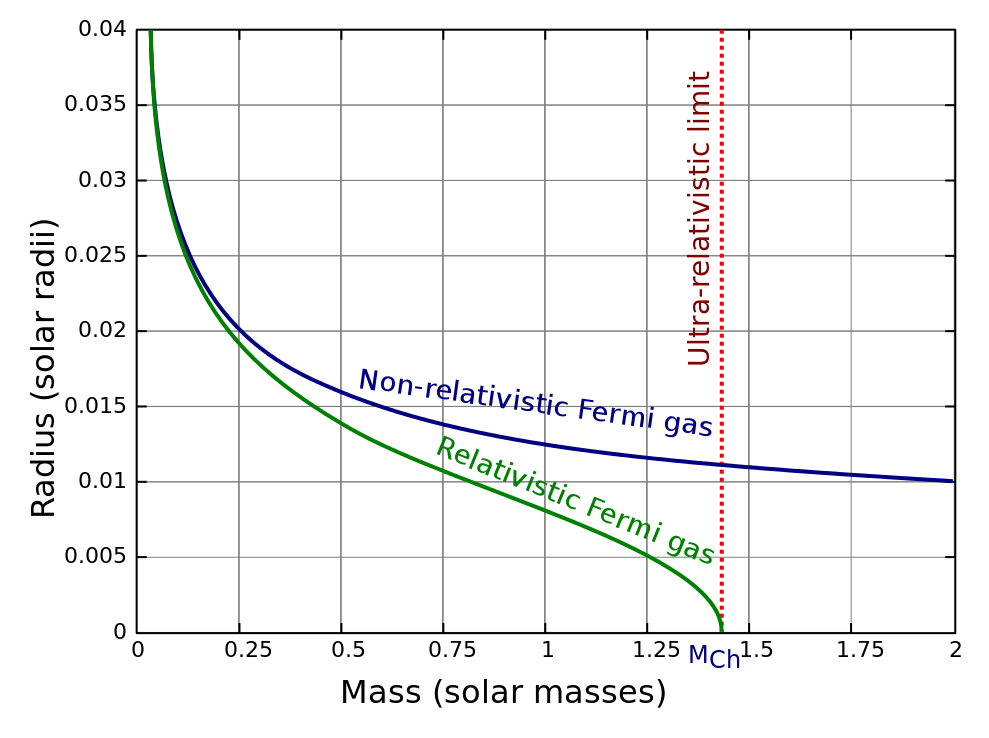
\includegraphics[scale=0.4]{chandra.png}
			\label{chandra}
		\end{figure}
	
		\noindent Questi due limiti sono entrambi poco realistici. Effettivamente, abbiamo trascurato del tutto le interazioni tra elettroni, che diventano importanti per basse densità (e quindi nel limite di piccola massa). Un grafico più realistico partirebbe a $M=0$ da $R=0$, poi crescerebbe fino a un certo valore, per poi seguire la curva teorica. Viceversa, per masse molto vicine al limite di Chandrasekhar l'impulso di Fermi cresce. Se supponiamo che la stella sia composta unicamente da protoni e elettroni, prima o poi $p_F$ supera il valore di soglia per la reazione
		\[\textrm{p + e}^-\to \textrm{n + }\nu\]
		detto processo $\beta$ inverso. Di conseguenza, esistenza una densità critica ($\rho_c\simeq 1.2\cdot10^7$ g/cm$^3$) oltre la quale la stella collassa, perchè la produzione di neutroni riduce il numero di elettroni, e quindi diminuisce la pressione di degenerazione che regge il sistema. In una stella vera, il valore della densità critica è più alto ($\rho_c\sim10^9$ g/cm$^3$), perchè sono presenti anche altri elementi.
		\item Ci sono diversi tipi di nane bianche, a seconda della massa iniziale della stella. Come già visto, se $M\leq 0.08M\s$ non si innesca alcuna reazione, e si forma una nana bruna. Se inve $0.08M\s\leq M\lesssim0.5M\s$, la stella non innesca la combustione dell'elio, alla fine della sequenza principale perde parte dell'inviluppo e comincia a raffreddarsi a raggio costante. Se $0.5M\s\lesssim M\lesssim 7-8M\s$ non si innesca la combustione del carbonio, e otteniamo una nana bianca a carbonio e ossigeno. Infine, per $M\gtrsim 10M\s$ la stella diventa una supernova. Le nane bianche più comuni oggi sono quelle a carbonio e ossigeno, infatti il tempo evolutivo decresce con $M$: se $M\leq M\s$, il tempo evolutivo è maggiore della vita dell'Universo, quindi le nane bianche a elio sono piuttosto rare oggi (e quelle che vediamo sono dovute a fenomeni anomali di "strappo di massa"). La perdita dell'inviluppo è in genere consistente: una nana bianca a C/O è composta usualmente per il 98-99\% da un nucleo di carbonio e ossigeno, mentre il restante 1-2\% è formato da un sottile strato superficiale di elio, circondato da uno strato ancor più sottile di idrogeno (che forma circa lo 0.1-0.01\% della massa del sistema). Quasi tutto il nucleo è quasi completamente degenere, mentre il sottile strato di idrogeno, almeno nelle prime fasi, non lo è completamente. Questo strato regola il rilascio di energia termica nell'ambiente circostante, mentre all'interno il trasporto è conduttivo.
		\item Vediamo ora un modello semplificato per il trasporto, dovuto a Mestel. Ricordiamo l'equazione di struttura per la luminosità
		\begin{align*}
		\der{L}{m}&=\varepsilon_N+\varepsilon_G-\varepsilon_\nu
		\end{align*}
		Assumiamo che
		\begin{enumerate}
			\item $\varepsilon_N=0$, ossia che non si siano reazioni. Se ci fossero, avremmo un flash che probabilmente farebbe esplodere tutta la struttura in una supernova.
			\item $\varepsilon_\nu=0$, ossia non c'è perdita di energia dovuta ai neutrini.
			\item La nana è incompribile.
			\item I nuclei sono classici e non degeneri, quindi il loro contributo al calore specifico è
			\[C_{V,i}=\frac{3N_Ak}{2A}\]
			\item Il contributo al calore specifico degli elettroni è dovuto essenzialmente agli elettroni con un'energia circa uguale a quella di Fermi, ovvero
			\[C_{V,e}=\frac{3N_Ak}{2A}\frac{\pi^2Z}{3}\frac{kT}{\varepsilon_F}\ll C_{V,i}\]
			\item La temperatura è uniforme.
		\end{enumerate}
		Dalle prime due segue che
		\begin{align*}
			\der{L}{m}=-T\der{S}{t}\\
			L=-\int_{0}^{M}T\der{S}{t}\d m
		\end{align*}
		Inoltre, se $S=S(\rho,T)$, si ha
		\begin{align*}T\der{S}{t}&=\left.\pder{S}{\rho}\right|_{T}\dot{\rho}+\left.\pder{S}{T}\right|_{\rho}\dot{T}=\\&=C_V\der{T}{t}\end{align*}
		dove si è usata l'incomprimibilità della nana. Allora si ottiene
		\[L=-\int_{0}^{M}C_V\der{T}{t}\d m\]
		che ci dice che la nana bianca brilla a spese dell'energia termica, accumulata nel nucleo nelle fasi precedenti (mentre, in queste ultime, il nucleo era caldo per rimanere all'equilibrio). Vista l'ipotesi sui calori specifici e sull'uniformità di $T$, si ottiene
		\[L=-\frac{3N_AkM}{2A}\der{T}{t}\]
		ovvero il sistema si raffredda. Per maggiori dettagli sull'evoluzione temporale ci si dovrebbe occupare del piccolo strato esterno, in ogni caso il tempo scala è
		\[\tau\propto\frac{1}{A}\left(\frac{M}{M\s}\right)^{2/7}\left(\frac{L}{L\s}\right)^{-5/7}\]
		Discutiamo ora le approssimazioni fatte: la prima è buona, dato che le reazioni sono presenti al più nelle primissime fasi, e comunque per nane piccole. La seconda è una pessima approssimazione, dato che in realtà i neutrini sono il canale principale di perdita di energia. L'ipotesi di incomprimibilità è in genere buona, tranne al più nelle fase iniziale. Inoltre, i nuclei effettivamente rimangono classici, ma non sono considerabili un gas perfetto. Considerando il rapporto
		\[\Gamma=\frac{Z^2e^2}{AkT}\]
		se $\Gamma\ll 1$, si possono trascurare le interazioni tra i nuclei. Tuttavia, al diminuire di $T$ si ha un aumento di $\Gamma$. Quando $\Gamma\sim 1$ si ha una transizione gas-liquido, a cominciare dalle zone centrali del nucleo, mentre per $\Gamma\gtrsim 175$ il nucleo inizia a cristallizzare. Questa transizione rilascia calore latente, che va sommato all'energia termica. Quando il sistema scende sotto la temperatura di Debye dei nuclei, si ha $C_{V,i}\propto T^3$, quindi il raffreddamento accelera.
		\item Come ultima cosa sulle WD, chiediamoci perchè è importante osservarle. Innanzitutto, abbiamo visto che sono oggetti antichi, quindi ci danno informazioni sul passato dell'Universo. Inoltre, il modello per il raffreddamento è piuttosto semplice, dato che lega facilmente la luminosità al tempo scala. Questo permette di utilizzare le nane come indicatori di età, e sappiamo bene che la datazione è uno dei problemi principali dell'astrofisica.
		\item Passiamo al modello di Eddington, che ci permette di dare un limite superiore alla luminosità di una stella. Introduciamo il rapporto
		\[\beta=\frac{P_G}{P}\]
		dove $P_G$ è la pressione del gas e $P$ è la pressione totale. Ovviamente, se $P_R$ è la pressione di radiazione si ha
		\[1-\beta=\frac{P_R}{P}\]
		Supponiamo di avere un gas perfetto che sia anche un corpo nero, di modo che
		\begin{align*}
			P_G&=\frac{\rho kT}{\mu m_H}\\P_R&=\frac{a}{3}T^4
		\end{align*}
		Con facili calcoli si ottengono allora la temperatura $T$ e la pressione totale
		\begin{align*}T&=\left(\frac{1-\beta}{\beta}\right)^{1/3}\left(\frac{3\rho k}{a\mu m_H}\right)^{1/3}\\P&=\left(\frac{1-\beta}{\beta}\right)^{1/3}\left(\frac{3k}{a\mu^4m_H^4}\right)^{1/3}\rho^{4/3}\end{align*}
		Le equazioni precedenti costituiscono il modello standard di Eddington. Osserviamo che, nell'azzardata ipotesi che $\beta$ sia costante in tutta la struttura stellare, abbiamo una politropica con $n=3$, che corrisponde a un gas ultrarelativistico. Usiamo ora le equazioni di struttura, in particolare
		\begin{align*}
			\der{P}{r}&=-\frac{Gm\rho}{r^2}\\
			\der{P_R}{r}&=-\frac{\bar{k}\rho}{c}\frac{L}{4\pi r^2}
		\end{align*}
		Notando che
		\[\der{P_R}{P}=1-\beta\]
		si ottiene
		\[L=\frac{4\pi cGM}{\bar{k}}(1-\beta)\]
		Il valore massimo per $L$ è detto luminosità di Eddington, e si ha ovviamente per $\beta=0$
		\[L\leq L_{\textrm{max}}=\frac{4\pi cGM}{\bar{k}}\]
		Se in una stella $L\geq L_\textrm{max}$, "qualcosa" inizia a staccarsi. Più esplicitamente, se prendiamo una stella molto massiccia (ad esempio, con core di ferro), avvicinandosi alla massa di Chandrasekhar la densità aumenta. Raggiunta una certa soglia, si innescano dei processi di neutron drip, in cui i nuclei decadono emettendo neutroni. Questo fenomeno aumenta ulteriormente la densità e la pressione dei neutroni diventa a poco a poco dominante su quella degli elettroni degeneri. In contemporanea, si innesca anche la fotodisintegrazione del ferro, che libera nuclei di elio e altri neutroni. La stella va incontro a un collasso molto rapido, che crea una stella a neutroni (in cui la densità è dell'ordine delle densità nucleari, ossia $\rho\sim10^{14}$ g/cm$^3$). In ogni caso, anche per una stella a neutroni esiste una massa limite, ma il suo calcolo è ben più complicato rispetto alla massa di Chandrasekhar (principalmente a causa delle interazioni non più trascurabili). Nel 1967 arrivarono le prime evidenze sperimentali a favore dell'esistenza delle stelle a neutroni. Stimiamo ora l'energia liberata nel collasso di una nana bianca in una stella a neutroni. Consideriamo quindi una nana di massa $m\simeq 1.4M\s$ e raggio $R\simeq R_E$. Il raggio dopo il collasso è ben minore, stimabile con $R\simeq 10$ km. L'energia liberata è allora
		\[E\simeq GM^2\left(\frac{1}{R}-\frac{1}{R_E}\right)\simeq 10^{53}\textrm{ erg}\]
		In queste condizioni si ha $Mc^2\simeq10^54$ erg, dunque è assai probabile che ci siano effetti relativistici importanti. Nel 1977 venne scoperta la prima pulsar, ossia un oggetto astronomico che emette dei pulsi regolari, periodici e puliti. Il periodo era $T\simeq 1$ s, e aumenta lievemente nel tempo. Ovviamente, questo periodo pone un limite inferiore alla densità. Se $M$ e $R$ sono la massa e il raggio della struttura, deve aversi
		\[\left(\frac{2\pi}{T}\right)^2R\leq\frac{GM}{R^2}\]
		ossia
		\[\rho\geq\rho_c=\frac{3}{4\pi G}\left(\frac{2\pi}{T}\right)^2\]
		che dà il valore critico $\rho_c\simeq10^{8}$ g/cm$^3$. Sono state anche osservate delle pulsar con $T\simeq 1$ ms, per cui $\rho_c\simeq10^{14}$ g/cm$^3$. Si formularono diverse ipotesi sulla natura delle pulsar, le principali ipotizzavano che fossero delle oscillazioni di una stella (ma questa ipotesi va scartata, perchè le oscillazioni stellari sono in genere la sovrapposizione di tanti modi normali, quindi non osserveremmo un segnale pulito, e in più il periodo dovrebbe diminuire nel tempo) o un sistema binario (ma anche qui il periodo diminuisce, e in più le due stelle dovrebbero essere assai compatte). Alla fine, l'ipotesi delle stelle a neutroni venne accettata. I parametri tipici di una stella a neutroni sono $m\simeq1.4 M\s$, $R\simeq 10$ km, $\rho\simeq 10^{14}$ g/cm$^3$, $E_\textrm{grav}\simeq 0.2 Mc^2$, $g\simeq 2\cdot10^{14}$ cm/s$^2$. Negli anni '30, Baade e Zwicky propongono che le supernove sono associate alla creazione di una stella a neutroni: tale ipotesi è effettivamente verificata per alcuni tipi di supernove.
		\item Dagli anni '60 si iniziarono a osservare le sorgenti di raggi X. I primi oggetti osservati furono le sorgenti di X variabili: molte sorgenti sono sistemi binari, in cui la materia di una stella "piove" su una stella a neutroni. In questa pioggia, l'energia liberata da una particella di massa $m$ è circa
		\[E\simeq\frac{GMm}{R}\simeq 0.1-0.16 mc^2\]
		che è ben maggiore dell'energia liberata nelle reazioni nucleari. Se immaginiamo che la superficie si scaldi e emetta come un corpo nero, usando per la luminosità il valore $L\simeq 10^{37}$ erg/s si ottiene $kT\simeq 1$ keV, dunque effettivamente siamo nell'X. Il valore della luminosità è pressochè uguale in tutte le sorgenti variabili ed è con ottima approssimazione la luminosità di Eddington. Se, per semplicità, supponiamo che la "pioggia" sia composta da idrogeno ionizzato, allora
		\[\bar{k}=\frac{n_e\sigma_T}{\rho}\]
		dove $\sigma_T$ è la sezione d'urto di Thomson. Infatti, in presenza di idrogeno ionizzato ci sono molti elettroni liberi che fanno scattering. Usando $\sigma_T\simeq6.65\cdot10^{-25}$ cm$^2$ e $n_e=n_H=\rho/m_H$, si ottiene
		\[L_\textrm{max}=\frac{4\pi cGMm_H}{\sigma_T}\simeq10^{38}\textrm{ erg/s}\]
		Il tempo scala del processo è il tempo di free fall, dunque l'inviluppo "non si accorge della pioggia" e si scalda, fino a rendere efficace la fotodisintegrazione del ferro, ovvero
		\[\tensor[^{56}]{\textrm{Fe}}{}\textrm{ + }\gamma\rightarrow13\tensor[^{4}]{\textrm{He}}{}\textrm{ + 4n}\]
		La reazione è fortemente endotermica (circa 2 MeV per nucleone), e a un certo punto diventa efficace anche la fotodisintegrazine dei nuclei di elio. Se la densità raggiunge un certo valore critico, si genera un'onda d'urto che brucia l'inviluppo in tempi molto brevi. Quest'onda d'urto produce nuclei (in particolare, dato che nell'inviluppo ci sono atomi con $Z=N$, ci aspettiamo processi $R$ che formano $\tensor[^{56}]{\textrm{Ni}}{}$, che poi decade in $\tensor[^{56}]{\textrm{Co}}{}$ e infine in $\tensor[^{56}]{\textrm{Fe}}{}$) che vengono immessi nel mezzo interstellare. Si pensa inoltre che i neutrini giochino un ruolo molto importante nell'esplosione: l'energia assorbita è circa il 10\% di quella disponibile, quella irradiata circa l'1\%, mentre la restante va proprio nei neutrini. Supernove di questo tipo si dicono gravotermiche, dato che sono innescate da processi gravitazionali. L'emissione da parte dell'onda è inizialmente non nel visibile (a causa della temperatura elevata), poi con l'espansione la temperatura diminuisce e si arriva nel visibile. Quando iniziano i decadimenti dei nuclei di nichel e cobalto, l'emissione dipende dall'emissione dei decadimenti, dunque $\log L\propto -\lambda t$, con $\lambda$ costante di decadimento.
		\item Slide sulle supernove
	\end{itemize}
	\section{Mezzo interstellare e struttura della Via Lattea}
	\begin{itemize}
		\item Stimare le dimensioni della Via Lattea è cruciale per avere un'idea delle dimensioni del cosmo. Per stimarle, è abbastanza naturale fare dei conteggi stellari. Il primo a occuparsi di ciò fu Herschel, che assunse che tutte le stelle hanno luminosità uguale a quella di Sirio e che non ci sia assorbimento intermedio tra una stella e la Terra. Entrambe le assunzioni sono errate, ma riuscì comunque a capire che la Via Lattea è un disco sottile. Immagina anche che il Sole sia al centro, perchè la distribuzione di stelle dalla Terra appare isotropa. Nel 1918, Shapley intuisce che siamo invece in una posizione periferica della galassia. In particolare, osserva che gli ammassi globulari sono concentrati per lo più nella costellazione del Sagittario, dunque se questi sono distribuiti isotropicamente rispetto al centro della galassia anche quest'ultimo deve essere nella direzione del Sagittario. Shapley stima anche che il Sole si trova a 15 kpc dal centro, mentre oggi sappiamo che si trova a circa 8 kpc. Nel 1912, Henrietta Levitt trova una relazione che lega il periodo delle stelle variabili, ossia le stelle la cui luminosità varia con regolarità, alla loro luminosità. Per farlo, osserva le nubi di Magellano, ipotizzando che le stelle delle nubi siano approssimativamente alla stessa distanza dalla Terra.
		\item La galassia è essenzialmente un disco sottile, di raggio di circa 15 kpc e spessore di circa 100 pc. Al centro c'è un rigonfiamento, detto bulge galattico. Intorno al centro sono distribuiti, in simmetria sferica (quindi anche e soprattutto fuori dal disco) gli ammassi globulari, in una regione chiamata alone o sferoide. In tale reime ci sono anche le stelle di campo. Il Sole è relativamente periferico, a circa 8 kpc dal centro. Le ipotesi che vedevano il Sole al centro trascuravano l'assorbimento del mezzo interstellare, che impedisce di ricevere la luce dagli oggetti più lontani. Nel 1930 Trumpler intuisce la presenza del mezzo. Riesce infatti a legare le dimensioni angolari degli ammassi aperti con la loro luminosità. La diminuzione della dimensione angolare e diversa da quella che si avrebbe nel vuoto, inoltre cambia anche l'indice di colore. Effetivamente, in assenza del mezzo sappiamo che la magnitudine apparente e assoluta sono legate da
		\[m-M=-5+5\log d\]
		dove $d$ è la distanza in pc. In presenza di assorbimento si ha piuttosto
		\[m-M=-5+5\log d+A\]
		dove $A$ è detto estinzione e dipende dalla frequenza, in particolare l'assorbimento è maggiore per piccole lunghezze d'onda (da cui l'arrossamento dei cluster lontani osservato da Trumpler). L'arrossamento $E(B-V)$ è proprio dato da
		\[E(B-V)=B-V-(B-V)_0\]
		dove il secondo termine è il valore che si avrebbe in assenza di estinzione. Numericamente, si ha $A\simeq 1.5 d$ e $E(B-V)\simeq 0.5 d$, dunque il loro rapporto è circa $1/3$ e non dipende da $d$. Da qui si possono ricostruire alcune proprietà del mezzo, come composizione, dimensioni e temperatura. Un'ulteriore prova della presenza del mezzo viene dagli spettri delle stelle binarie, in cui alcune righe oscillano e alcune no (quelle relative al mezzo). Il mezzo può essere studiato sia attraverso le righe di assorbimento (ma presuppone la presenza di una sorgente posta dietro il mezzo) che attraverso le righe di emissione (ma la temperatura del mezzo, dell'ordine di 100 K, rende difficile questo approccio, dato che gli elettroni sono legati e quindi non fanno transizioni nel visibile, ammesso che le facciano). Partiamo dalle righe di assorbimento. Si ha
		\[\alpha_\nu=n\sigma\phi(\nu)\]
		dove $n$ è il numero di atomi per unità di volume, $\phi$ è il profilo di riga e
		\[\sigma=\frac{e^2f}{4\varepsilon_0m_ec}\]
		$f$ è detta forza dell'oscillatore. La profondità ottica è allora
		\[\tau_\nu=\frac{e^2}{4\varepsilon_0m_ec}f\phi(\nu)\int_{s_0}^{s}n\d s'\]
		Possiamo introdurre la densità di colonna $N$, data da
		\[N=\int_{s_0}^{s}n\d s'\]
		Si noti che stiamo trascurando del tutto l'emissione stimolata. Sappiamo che il suo effetto è modellizzabile moltiplicando $\alpha_\nu$ per il fattore $1-\exp(-h\nu/kT)$, ma alle temperature tipiche del mezzo si ha $h\nu/kT\simeq 10-100$, dunque l'effetto è del tutto trascurabile. L'equazione del trasporto per il puro assorbimento ci dà allora
		\[I_\nu(s)=I_\nu(s_0)\exp\left(-\frac{e^2f\phi(\nu)}{4\varepsilon_0m_ec}N\right)\]
		La larghezza equivalente è allora
		\begin{align*}
			W_\lambda&=\frac{\int I_C-I_\lambda\d\lambda}{I_C}=\\&=\frac{\lambda_0}{c}\int(1-e^{-\tau_\nu})\d\nu
		\end{align*}
		Il mezzo è tendenzialmente otticamente sottile, dunque approssimando l'esponenziale si ottiene
		\[W_\lambda\simeq\frac{\lambda_0}{c}\int\tau_\nu\d\nu=\frac{\lambda_0^2e^2N}{4\varepsilon_0m_ec^2}f\]
		dato che il profilo di riga è normalizzato. In particolare, $W_\lambda/\lambda_0$ è proporzionale a $\lambda_0Nf$. In realtà, in un grafico reale si ha una sorta di plateau per $\lambda_0Nf$, poichè in tale condizioni $1-I_\lambda/I_C$ è fin troppo vicino a 1. Vediamo invece cosa si può dire sull'emissione. L'emissione principale proviene dalla struttura iperfine dell'idrogeno e consiste in una riga a $\lambda=21$ cm. L'emissione è dovuta a uno split del fondamentale, causato dagli spin di elettrone e nucleo. La differenza di energia corrispondente è di circa $6\cdot10^{-6}$ eV. Il livello a energia più alta ha popolazione che è circa il triplo di quella nel livello a energia bassa (dato che $h\nu/kT\simeq0$ e $g_2=3$, $g_1=1$), ma la probabilità di transizione è assai bassa: si ha $A_{21}=2.85\cdot10^{-15}$ s$^{-1}$, dunque il tempo di decadimento del livello è di circa 11 milioni di anni. La grande quantità di idrogeno presente nel mezzo e la sua estrema rarefazione permettono comunque di osservare questi rari eventi. In realtà, in tali condizioni ci si può chiedere se sia possibile usare la distribuzione di Boltzmann. Infatti, a densità molto basse potrebbe essere importante anche il contributo della radiazione. Ricordiamoci dei risultati sui coefficienti di Einstein e sui coefficienti di emissione e assorbimento
		\begin{align*}
			g_1B_{12}&=g_2B_{21}\\
			A_{21}&=\frac{2h}{c^2}\nu^3B_{21}\\
			j_{\nu}&=\frac{h\nu}{4\pi}n_2A_{21}\phi(\nu)\\
			\alpha_\nu&=\frac{h\nu}{4\pi}\phi(\nu)n_1B_{12}\left(1-e^{-h\nu/kT}\right)
		\end{align*}
		Se immaginiamo invece di avere un sistema a due livelli con processi di assorbimento, emissione e collisioni, in condizioni stazionarie dobbiamo avere
		\[n_1\left(B_{12}\bar{J}+\gamma_{12}n_e\right)=n_2(A_{21}+B_{21}\bar{J}+\gamma_{21}n_e)\]
		dove $\gamma_{ij}$ è il rate di eccitazione dallo stato $i$ allo stato $j$ a causa delle collisioni e $n_e$ è la densità elettronica. Al solito, se siamo all'LTE si ha
		\[\bar{J}=\frac{2h\nu^3}{c^2}\frac{1}{e^{h\nu/kT}-1}\]
		e se supponiamo che valga la distribuzione di Boltzmann si ha anche
		\[g_1\gamma_{12}=g_2\gamma_{21}e^{-h\nu/kT}\]
		Perturbativamente, si ricava il rapporto tra le popolazioni
		\[\frac{n_2}{n_1}=\frac{g_2}{g_1}e^{-h\nu/kT}\frac{1}{1+\frac{A_{21}}{\gamma n_e}}\]
		Effettivamente, Boltzmann è un'approssimazione accettabile se siamo a densità superiori a una certa soglia (convenzionalmente $n_e\leq A_{21}/\gamma_{21}$). In caso contrario, la popolazione del livello più alto è minore di quanto previsto da Boltzmann. Nel nostro caso la densità critica è dell'ordine $n_e\simeq 10^{-5}$ at/cm$^3$, dunque la statistica di Boltzmann è adeguata nella trattazione del mezzo interstellare. Notiamo incidentalmente che se $n_2B_{21}>n_1B_{12}$ il mezzo si comporta come un maser, dato che il coefficiente di assorbimento è negativo. Ricordiamoci ora che per un mezzo sottile si ha
		\[I_\nu=\int j_\nu\d s\]
		In tal modo, si ha per l'intensità
		\begin{align*}
			I&=\int I_\nu\d\nu=\\&=\int\d s\int\d\nu\frac{h\nu}{4\pi}\phi(\nu)n_2A_{21}\simeq\\&\simeq \int\d s\frac{h\nu_0}{4\pi}n_2A_{21}=\frac{3h\nu_0}{16\pi}A_{21}N
		\end{align*}
		dove si è tenuto conto che $g_2=3g_1$, dunque $n_2=3n/4$. Allora, come già anticipato, se $N$ è sufficientemente elevato è possibile avere un valore rilevante per $I$. Osserviamo inoltre che $I$ non dipende dalla temperatura. In tal modo è possibile trovare l'abbondanza di idrogeno neutro. Per trovare la temperatura, possiamo utilizzare nuovamente l'assorbimento. Sappiamo che si ha ($h\nu/kT\ll 1$)
		\begin{align*}\alpha_\nu&=\frac{h\nu}{4\pi}\phi(\nu)n_1B_{12}=\\&=\frac{(h\nu)^2}{4\pi}\phi(\nu)n_1\frac{c^2A_{21}}{2h\nu^3}=\\&=\frac{c^2A_{21}n}{32\pi kT}\frac{\phi(\nu)}{\nu}\end{align*}
		dove si è usato il fatto che $n_1=n/4$ (ma a quanto pare pgpm mette per motivi oscuri un 3 a numeratore nell'ultima espressione). In tal modo, la profondità ottica è
		\[\tau_\nu=\frac{3hc^2A_{21}\phi(\nu)}{32\pi k\nu}\int_{0}^{s}\frac{n}{T}\d s'\]
		Dunque un'analisi opportuna della profondità ottica permette di ricostruire anche il profilo di temperatura. In tal modo si è scoperto che esistono zone a 8000 K (queste zone sono decisamente meno opache rispetto all'ambiente circostante) (DISCORSO A CASO SU DUE RIGHE SOVRAPPOSTE). Dall'effetto Doppler è anche possibile studiare la dinamica del mezzo.
		\item I bracci di spirale della Via Lattea sono dovuti a una distribuzione del mezzo non omogenea nel disco galattico, e sono stati visti tramite l'idrogeno neutro. Sono anche presenti delle nubi molecolari, in cui le particelle hanno molti più livelli energetici. Si ipotizza che le molecole si formino sulla superficie dei grani di polveri del mezzo. Le molecole principali sono H$_2$, ma la sua presenza è difficilmente rilevabile (non ha un momento di dipolo intrinseco, quindi può essere rilevato solo tramite l'assorbimento), CO (che ha emissioni forti, corrispondenti a una temperatura di corpo nero di $10^9$ K, dovute a transizioni rotazionali, a $\lambda_0=2.6$ mm e sottomultipli), OH, H$_2$O, NH$_3$, CH$_4$, e anche alcool etilico e glicina. Le nubi molecolari sono concentrate più verso il centro del disco. Le emissioni così forti sono dovute a un'inversione dei livelli. L'inversione è causata dal fatto che sulle nubi incide una radiazione esterna intensa nella regione dell'infrarosso, generata tipicamente nelle zone di formazione stellare. Questa radiazione scalda la materia, che comincia a emettere nell'infrarosso. In altri casi, l'inversione è realizzata da nuclei galattici attivi: si forma un disco di accrescimento intorno a un buco nero supermassiccio che scalda la polvere circostante. Infine, il mezzo che circonda stelle calde può anche essere ionizzato, e dunque può emettere nel visibile.
		\item Baade propone la seguente classificazione stellare
		\begin{itemize}
			\item Popolazione II: sono le stelle con caratteristiche simili alle stelle presenti nell'alone, dunque sono stelle antiche (circa 12 miliardi di anni), di prima generazione, con bassa metallicità (circa $10^{-3}-10^{-4}$).
			\item Popolazione I: sono le stelle con caratteristiche simili alle stelle presenti nel disco, dunque ci sono diverse generazioni e età stellari, la metallicità è relativamente alta ($Z\sim0.015$)
		\end{itemize}
		Inoltre, nel disco è presente molto mezzo interstellare, formato sia da grani di polvere che da gas (principalmente idrogeno neutro). La temperatura media del mezzo è 80-100 K, con alcune zone che raggiungono gli 8000 K, mentre la densità è dell'ordine di 1-100 at/cm$^3$. Nelle nubi molecolari invece si ha $T\sim 30-50$ K e $\rho\sim 10^3-10^4$ at/cm$^3$. In queste regioni si formano le stelle, in particolare il mezzo che circondata una stella appena nata è ionizzato. Stromgren è il primo a modellizzare la sfera che porta il suo nome, assumendo che la luminosità stellare sia costante durante la formazione e che il mezzo sia omogeneo. Supponiamo quindi che ci sia una sfera di raggio $R$ di H-II intorno a una stella, mentre all'esterno di tale sfera ci sia H-I. Il cammino libero medio di un fotone ionizzante è $l=1/n\sigma$, con $n$ densità di idrogeno e $\sigma$ sezione d'urto di Thomson (dato che abbiamo elettroni liberi). Usualmente si ha $n\simeq 10^3$ cm$^{-3}$ e $\sigma=6.65\cdot10^{-25}$ cm$^2$, dunque $l\simeq1.5\cdot10^{19}$ cm. Se il fotone raggiunge una distanza $R$ dalla stella, la sezione d'urto cambia (dato che qui sono presenti atomi neutri che possono essere ionizzati) e si ha $l\simeq10^{14}$ cm. Assumiamo quindi che se un fotone raggiunge la il bordo della sfera interagisca sicuramente. Il numero di fotoni ionizzanti può variare sia a causa di un'interazione al bordo della sfera, sia a causa della ricombinazione. Allora se $N_i$ è il loro numero all'interno della sfera, si deve avere
		\[\der{N_i}{t}=-4\pi R^2n\der{R}{t}+\frac{4\pi}{3}R^3 n_pn_e\alpha(T)\]
		dove $n_p$ e $n_e$ sono le densità di protoni e di elettroni e $\alpha$ è il coefficiente di ricombinazione, ossia $\alpha=\langle\sigma,v\rangle$. All'equilibrio si ha dunque
		\[\der{N_i}{t}=\frac{4\pi}{3}R^3n_pn_e\alpha(T)\]
		Il raggio della sfera di Stromgren è allora
		\[R=\left(\frac{3}{4\pi n_en_p\alpha}\der{N_i}{t}\right)^{1/3}\]
		Se $L_\nu$ è la luminosità associata alla frequenza $\nu$ e $\bar\nu=13.6\textrm{ eV}/h$, si ha
		\[\der{N_i}{t}=\int_{\bar\nu}^{\infty}\frac{L_\nu}{h\nu}\d\nu\]
		dunque è possibile calcolare $R$ una volta che conosciamo lo spettro della stella. Tipicamente si ha $\d N_i/\d t\simeq3\cdot10^{49}$ s$^{-1}$, $n_p\sim n_e\sim n$, da cui $R\sim$. Il valore così ottenuto è in realtà un limite inferiore al raggio, perchè la ricombinazione emette un fotone ionizzante solo se la transizione è dallo stato libero al fondamentale.
	\end{itemize}
\end{document}